% !Mode:: "TeX:UTF-8"
%% !TEX program  = xelatex
%! TEX program = xelatex
%\documentclass{cumcmthesis}
\documentclass[withoutpreface,bwprint]{cumcmthesis} %去掉封面与编号页,电子版提交的时候使用。
\usepackage{etoolbox}
\BeforeBeginEnvironment{tabular}{\zihao{-5}}
\usepackage{cite}
\usepackage[numbers,sort&compress]{natbib}
\usepackage[framemethod=TikZ]{mdframed}
\usepackage{url}   % 网页链接
\usepackage{subcaption} % 子标题
\title{基于一维热传导的炉温曲线模拟与优化}
\tihao{A}
\baominghao{4321}
\schoolname{华南理工大学}
\membera{ }
\memberb{ }
\memberc{ }
\supervisor{ }
\yearinput{2020}
\monthinput{08}
\dayinput{22}
\usepackage{yhmath}
\graphicspath{{figures/}}



\begin{document}

	\maketitle
	\begin{abstract}
		炉温曲线的控制决定了电子元件焊接的产品质量,本文基于一维热传导方程和牛顿冷却定律建立了炉温曲线变化规律的机理模型。
		
		\textbf{对于问题一,}首先基于热传导方程,推导出温区间隙之间温度线性过渡,建立回焊炉内部的温度分布模型。再通过\textbf{热传导方程与牛顿冷却定律},建立焊接区域的温度分布模型,边界条件为第三类边界条件,建立微分控制方程组(包含6个待求参数,5个$\alpha$,1个$\beta$)。利用\textbf{有限差分法}对方程组逐层求解,基于\textbf{最小二乘原理},拟合实测温度,遍历得到最优的参数组合,其中最优$\alpha$为$[3.78E-07, 4.95E-07 , 5.71E-07, 4.74E-07,  2.10E-07 ]cm^2/s$,最优$\beta$为$82197 cm^{-1}$。拟合数据与实际数据的\textbf{$\bm{R^2}$为0.9997},拟合效果较优。将求得的未知参数及问题一相关参数代入方程求解,得到炉温曲线,其中小温区3、6、7中点及小温区8结束处焊接区域中心的温度分别为\textbf{	129.2787$\bm{^\circ C }$ , 168.2546$\bm{^\circ C}$  , 189.1527$\bm{^\circ C}$   , 231.5747$\bm{^\circ C}$ },每隔0.5 s焊接区域中心的温度存放在result.csv中。
		
		\textbf{对于问题二,}建立以最大过炉速度为目标的\textbf{单目标优化模型}。以制程界限为约束条件。对约束条什进行差分,得出差分后的约束条件。应用问题一中得出的热传递模型,并利用\textbf{变范围搜索}的方法,搜索该温度分布条件下最大速度为$\bm{78.95cm/min}$.
		
		\textbf{对于问题三,}根据问题三的要求与制程界限约東,将该问题转换为关于温区温度和过炉速度的,以面积最小化为目标的单目标多变量最优化问题,并使用\textbf{遗传算法}求解。本文进行了多次独立求解,在多次结果中取最优的结果。最终确定的最佳变量值为$\bm{182.1140^\circ C} $(小温区1-5),$\bm{189.8592^\circ C }$(小温区6),$\bm{230.2581^\circ C }$(小温区7),$\bm{264.9846^\circ C} $(小温区8-9),过炉速度为$\bm{91.5834cm/min}$,阴影部分面积为$\bm{488.2102(^\circ C \cdot s)}$.
		
		\textbf{对于问题四,}同样根据多种约束,建立以\textbf{面积最小化}和\textbf{对称性指标最小化}为目标的多目标多变量最优化问题,利用遗传算法,结合\textbf{分层序列法}的思想,先优化面积指标,再优化对称性指标,多次求解得到多组求解结果,并取最优结果,最佳变量值为$\bm{172.3431^\circ C }$(小温区1-5),$\bm{185.0034^\circ C} $(小温区6),$\bm{230.637^\circ C }$(小温区7),$\bm{265.00^\circ C }$(小温区8-9),过炉速度为$\bm{88.7126cm/min}$,其中面积指标为$\bm{487.2066(^\circ C \cdot s)}$,对称性指标为$\bm{9.3831(^\circ C )}$。
		
		最后,本文对相关参数进行了\textbf{灵敏性分析},并对模型作出了评价。
		
		
		
		\keywords{一维热传导\quad  参数拟合\quad  有限差分法\quad  变范围搜索 \quad  分层序列法 \quad  遗传算法}
	\end{abstract}
	
	%目录  国赛不要求目录
	%\tableofcontents
	
	%\newpage
	
	\section{问题重述}
	\subsection{问题背景}
	为了生产集成电路板,将安装有电子元件的电路板置于回焊炉中,通过高温空气加热后元件被焊接在电路板上。回焊炉内有几个小温区,以功能上划分为4大温区:预热区、恒温区、回流区、冷却区。电路板搭在传送带上匀速进入炉内进行焊接。
	
	某回焊炉内有炉前区域和炉后区域和11个小温区。小温区长为30.5 cm,相邻小温区间隔2cm,炉前和炉后区域长为25 cm。启动回焊炉后,短时间内炉内空气温度达到稳态。生产车间的温度保持在25ºC。
	
	通过装载在电路板中心的热电偶等装置,可以测试焊接区域中心的温度,即炉温曲线。附件给出了某次实验数据,在本次实验中,各温区设定的温度分别为175ºC、195ºC、235ºC、255ºC及25ºC,传送带速度为70cm/min,焊接区域厚为0.15 mm。传感器在温度大于30ºC时开始工作,电路板进入炉前区域时,开始计时。
	
	通过改变各温区的温度以及传送带速度,可以控制产品质量。以本次实验温度为基础,各温区的温度能够在±10ºC范围内进行调整,并且要求温区1-5的温度相同,温区8-9中温度相同,温区10-11温度保持25ºC。传送带速度范围为65-100 cm/min。同时在电路板焊接生产过程中,炉温曲线应满足制程界限,例如上升下降斜率不能大于3等等。
	\subsection{问题要求}
	
	\textbf{问题1}  首先建立炉温曲线的模型。在此基础上,传送带速度变为78 cm/min,各温区温度相应地改变为为173ºC、198ºC、230ºC和257ºC,要求求出该情况下的炉温曲线,列出小温区3、6、7中点及小温区8结束炉温曲线温度。还需要将每隔0.5 s焊接区域中心的温度存放在result.csv中。
	
	\textbf{问题2}  各温区温度变成为182ºC、203ºC、237ºC、254ºC,求解允许的最大过炉速度。
	
	\textbf{问题3} 炉温曲线超过217ºC的时间不能过长,峰值温度也不能过高,超过217ºC到峰值温度所覆盖的面积应该最小。求解该要求下的最优炉温曲线,以及各温区温度和过炉速度,并计算相应的面积指标。
	
	
	\textbf{问题4}  在高温焊接过程中,除了需要满足制程界限,还要求以峰值温度为中心线的两侧超过217ºC的炉温曲线尽量对称。在问题3的基础上,给出最优炉温曲线以及各温区温度及过炉速度,同时给出相应的面积指标值和对称性指标值。
	
	
	\section{问题分析}
		\subsection{问题一分析}
		对于问题一,首先基于热传导方程,推导出温区间隙之间温度线性过渡,建立回焊炉内部的温度分布模型。再通过热传导方程与牛顿冷却定律,建立焊接区域的温度分布模型,边界条件为第三类边界条件,建立微分控制方程组。基于最小二乘法,利用附件数据进行参数拟合,得到误差最小时最优参数。带入问题一中给出的回焊炉各温区的温度数据,得出焊接处中心温度随时间变化的情况。
		
		\subsection{问题二分析}	
		对于问题二,在题目给定的温度条件和制程界限的限制下,求解最大化传送带速度的单目标规划模型。基于问题一中得出的炉温曲线模型,利用变范围搜索方法,对传送带的可能速度进行多次遍历,以得出精度较高的解。取$1cm/min$ 的速度步长,从$60cm/min$往上遍历后选取出第一个满足制程界限的解,即为最大解。
		
		\subsection{问题三分析}
		对于问题三,根据问题要求与制程界限约東,将该问题转换为关于温区温度和过炉速度的单目标多变量最优化问题,求出最优的温区设定温度和传送带的过炉速度,使得在满足制程界限的同时,炉温曲线超过217℃到峰值温度所覆盖的面积也达到最小。由于参数过多,遍历搜索的难度极大,可以考虑采用遗传算法等智能算法求解。
		
		\subsection{问题四分析}
		问题四是在问题三基础上的多目标优化问题,需要满足制程界限的同时,在问题三炉温曲线超过217℃到峰值温度所覆盖的面积达到最小的基础上,做到以峰值温度中线的两侧超过217℃的炉温曲线尽量对称的目标。因此建立以面积最小化和对称性指标最小化为目标的多目标多变量最优化问题,利用遗传算法,结合分层序列法的思想,先优化面积指标,再优化对称性指标,最终求得最佳参数。
		
	
	
	\section{模型假设}
	
	\begin{itemize}
		\item 元件在传送带上运行时与小温区始终保持垂直。
		\item 回焊炉内温度稳定,只在沿传送方向上变化,垂直于传送方向的平面温度稳定。
		\item 假设元件为材质处处均匀的带厚度无限大平板,内部不含热源
		\item 仅考虑热传导和热对流对元件焊接区域中心温度的影响
	\end{itemize}
	
	\section{符号说明}
% Table generated by Excel2LaTeX from sheet 'Sheet1'
\begin{table}[htbp]
	\centering
	\begin{tabularx}{\textwidth}{@{}l *2{>{\centering\arraybackslash}X}@{}}
	\toprule[1.5pt]
		符号    & 说明    & 单位 \\
		\midrule
		$l     $& 小温区长度 & $cm$ \\
		$a     $& 小温区间隔 & $cm$ \\
		$b     $& 炉前炉后区域长度 & $cm$ \\
		$d     $& 电路板厚度 & $cm $\\
		$t     $& 时间    & $s$ \\
		$u(x,t)$ & 电路板各处温度分布 & - \\
		$u(t)  $& 电路板中心温度随时间的变化(炉温曲线) & - \\
		$u_s(t) $& 空气温度随时间的变化 &  -\\
		$T_{15}   $& 小温区1-5设定温度 & $^\circ C $ \\
		$T_{06}  $& 小温区6设定温度 & $^\circ C $ \\
		$T_{07}   $& 小温区7设定温度 &  $^\circ C $\\
		$T_{89}   $& 小温区8-9设定温度 &  $^\circ C $\\
		$T_{1011} $& 小温区10-11设定温度 &  $^\circ C $\\
		$v     $& 传送带过炉速度 & $cm/s$\\
		$S     $& 问题3、4的面积指标 &  $(^\circ C \cdot s)$\\
		$D     $& 问题4对称性指标 &  $(^\circ C )$ \\
		\bottomrule[1.5pt]
	\end{tabularx}%
	\label{tab:addlabel}%
\end{table}%


	
	\section{模型的建立和求解}
	\subsection{炉内温度随位置的变化}
	问题一中,由题可知,炉内空气温度会在短时间内达到稳定,因此首先要建立稳态时回焊炉中空气温度随位置分布的规律。对于空气温度随$u_s(x)$,在热导率一定时,根据热导微分方程式,有
	\begin{align}
	\frac{\partial u_s(x)}{\partial t}=\alpha\frac{\partial^2u_s(x)}{\partial x^2}
	\label{wt}
	\end{align}
	对于稳态温度场,有$\frac{\partial u_s(x)}{\partial t}=0$,因此$\alpha\frac{\partial^2u_s(x)}{\partial x^2}=0$,小温区内空气温度等于设置温度,对于小温区间隙中的温度,对式(\ref{wt})积分,有
	\begin{equation}\label{key}
	u_s(x)=k_1 x+b_1
	\end{equation}
	即小温区间隙中的温度随着空间均匀变化,线性地由上一台阶温度过渡到下一台阶温度。
	
	设炉前炉后距离为$b$,各小温区的间距为$a$,各小温区的长度为$l$,令各分割点的位置为
	\begin{equation}\label{wqwz}
	\begin{cases}
	len0=b\\
	len1=b+5l+4a\\
	len2=b+5l+5a\\
	len3=b+6l+4a\\
	len4=b+6l+6a\\
	\end{cases}\,\,   \begin{cases}
	len5=b+7l+6a\\
	len6=b+7l+7a\\
	len7=b+9l+8a\\
	len8=b+9l+9a\\
	len9=b+11l+10a+b\\
	\end{cases}
	\end{equation}
	则空气温度$U_s(x)$关于距离$x$的分段函数为:
	\begin{equation}\label{usx}
	U_s\left( x \right) =\left\{
	\begin{array}{lcl}
	
	\frac{T_{15}-25}{len0} x+\text{25  }& &0<x\leqslant len0\\
	
	T_{15}& &len0<x\leqslant len1\\
	
	\frac{T_{06}-T_{15}}{len2-len1}(x-len0)+T_{15}& &len1<x\leqslant len2\\
	T_{15}& &len2<x\leqslant len3\\
	
	\frac{T_{07}-T_{06}}{len4-len3}(x-len3)+T_{06}& &len3<x\leqslant len4\\
	T_{07}& &len4<x\leqslant len5\\
	
	\frac{T_{89}-T_{07}}{len6-len5}(x-len5)+T_{07}& &len5<x\leqslant len6\\
	T_{89}& &len6<x\leqslant len7\\
	
	\frac{T_{1011}-T_{89}}{len8-len7}(x-len7)+T_{15}& &len7<x\leqslant len8\\
	T_{1011}& &len8<x\leqslant len9
	\end{array} \right.
	\end{equation}
	其中$T_{15}$是小温区1-5的温度,$T_{06}$是小温区6的温度,$T_{07}$是小温区7的温度,$T_{89}$是小温区8-9的温度,$T_{1011}$是小温区10-11的温度。
	
	考虑到传送带是匀速运动的,电路板的位移$x=vt$,模型中讨论的电路板周围空气温度可以看作是随时间变化的量,空气温度随时间的变化函数$u_s(t)$可以写作$U_s(vt)$。
	\begin{equation}\label{vt}
	u_s(t)=U_s(x)=U_s(vt)
	\end{equation}
	传送带运动速度为$70cm/s$,在此速度下回焊炉中的温度随时间(位置)变化如图示
	\begin{figure}[H]
		\centering
		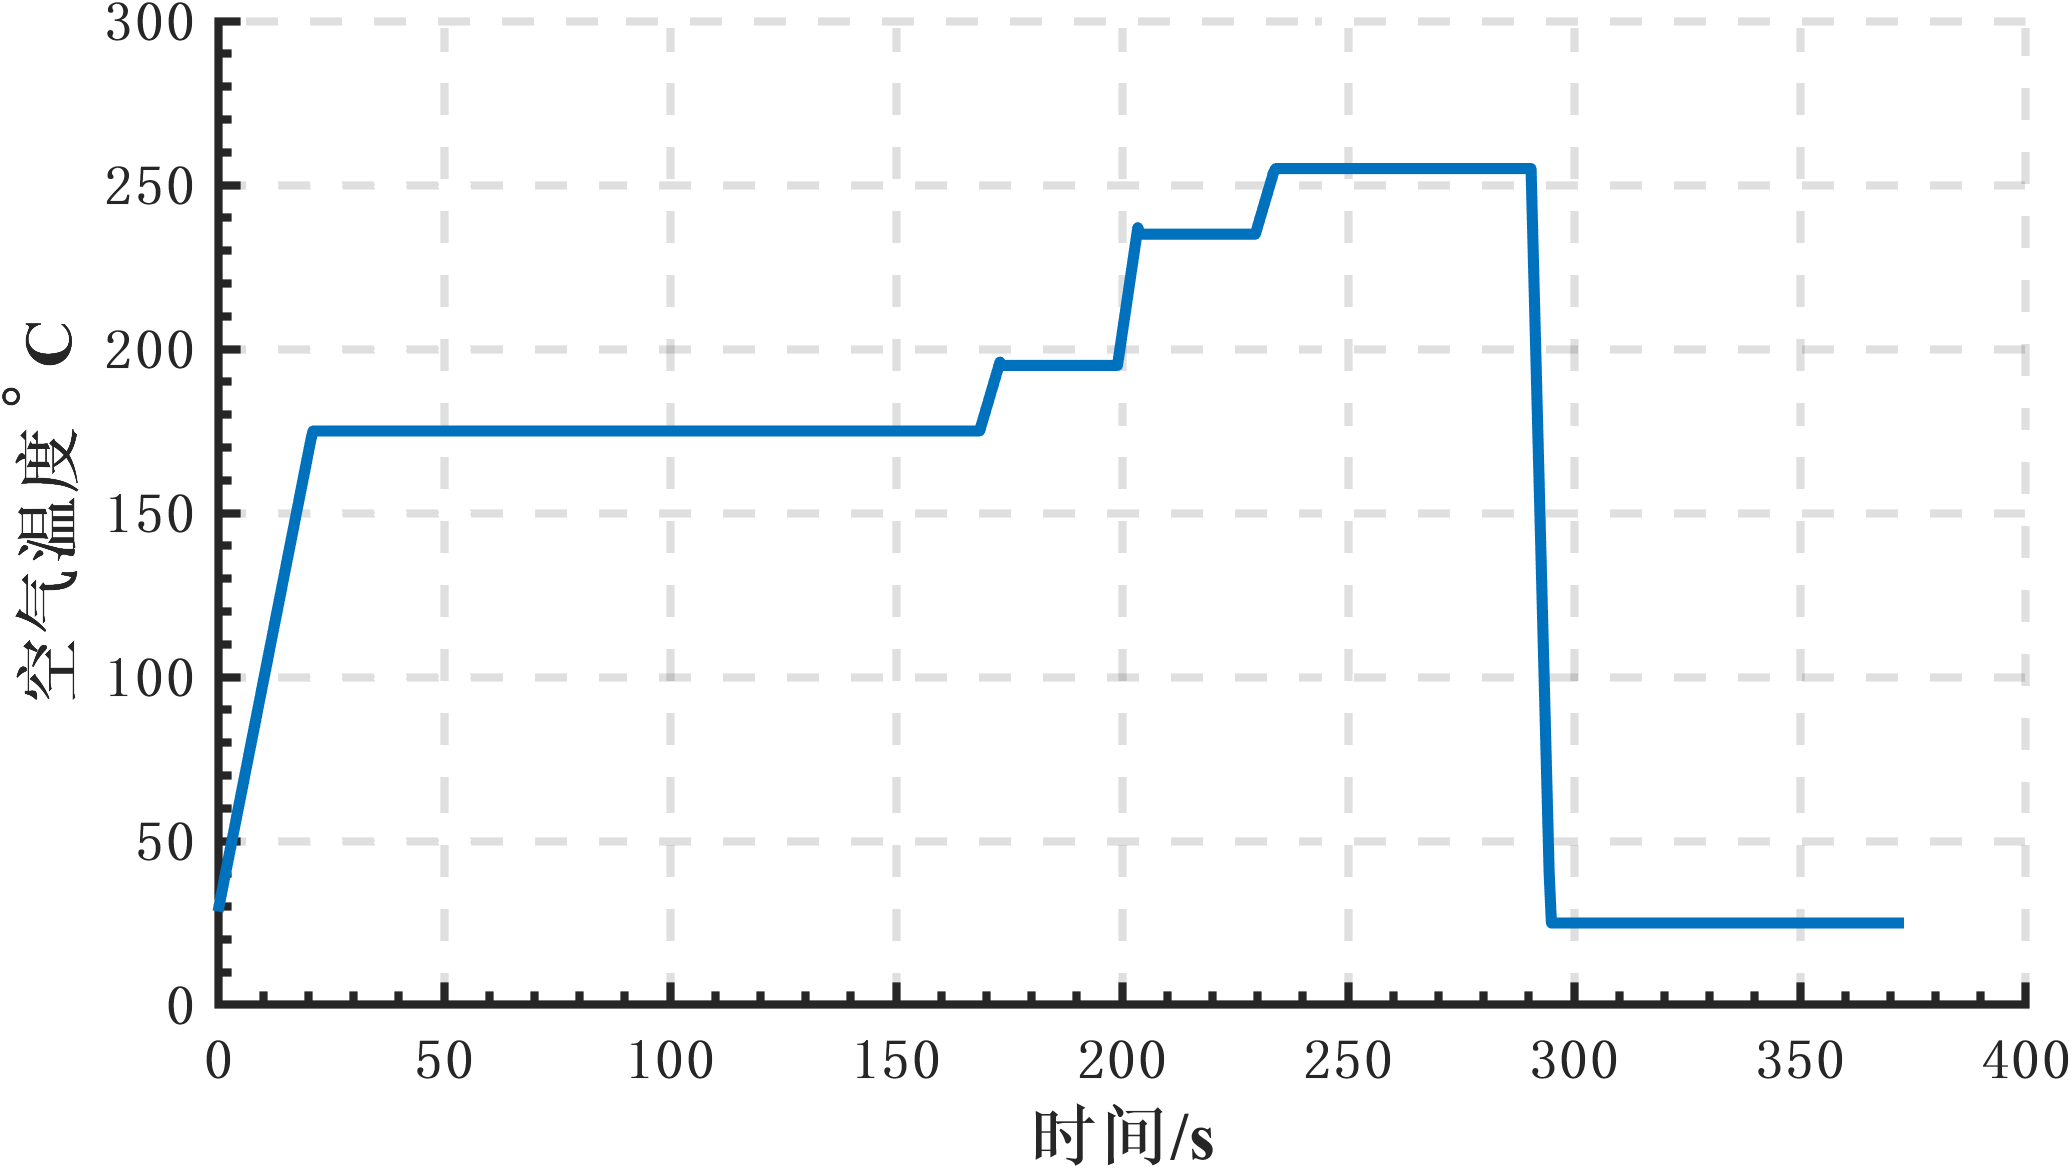
\includegraphics[width=0.6\textwidth]{空气温度趋势图.png}
		\caption{回焊炉温度随时间(位置)的变化}\label{空气温度趋势图}
	\end{figure}
	
	\subsection{电路板上一维热传导模型的建立}
	
	对于电路板上的温度$u(x,t)$,以电路板下端中心为原点建立坐标轴,方向向上为正:
	\begin{figure}[H]
		\centering
		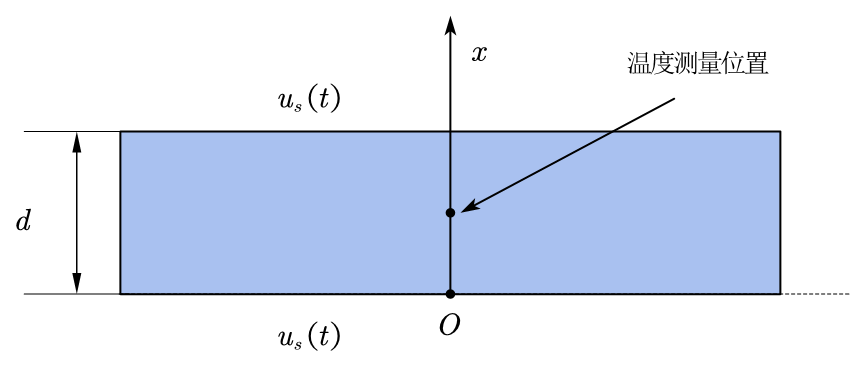
\includegraphics[width=0.8\textwidth]{电路板示意图.png}
		\caption{电路板示意图}\label{电路板示意图}
	\end{figure}
	同样根据热导微分方程式,得到控制方程
	\begin{align}
	\frac{\partial u(x,t)}{\partial t}=\frac{\lambda}{c\rho}\frac{\partial^2u(x,t)}{\partial t^2}
	\end{align}
	其中$\lambda$为热导率,$c,\rho$分别为比热容与密度。
	在电路板的上下边界上,满足第三类边界条件,根据牛顿冷却公式,物体边界面与流体对流换热量可以写为$q=h(u-u_s(t))$,其中$h$为边界面与空气的表面传热系数,$u_s(t)$为空气温度。则对于电路板的上下边界有
	\begin{equation}
	\left\{
	\begin{array}{rcl}
	
	&&\lambda\frac{\partial u}{\partial x}|_{x=d}=h(u_s(t)-u(d,t)) \\
	&&-\lambda\frac{\partial u}{\partial x}|_{x=0}=h(u_s(t)-u(0,t)) 
	
	\end{array} \right.
	\end{equation}
	上述公式中,令$\alpha=\frac{\lambda}{\c\rho}$,$\beta=\frac{h}{\lambda}$,得到
	\begin{equation}
	\left\{
	\begin{array}{rcl}
	&&\frac{\partial u(x,t)}{\partial t}=\alpha\frac{\partial^2u(x,t)}{\partial x^2}  \\
	&&\frac{\partial u}{\partial x}|_{x=d}=\beta(u_s(t)-u(d,t))  \\
	&&-\frac{\partial u}{\partial x}|_{x=0}=-\beta(u_s(t)-u(0,t))  
	\end{array} \right.
	\label{lfc}
	\end{equation}
	\subsection{有限差分法求解热方程}
	对式(\ref{lfc})离散化,其中边界条件离散为
	\begin{equation}
	\label{bjtjls}
	\begin{aligned}
	&-\frac{u_{2, j+1}-u_{1, j+1}}{\Delta x}=\beta\left(u_{s}(j+1)-u_{1, j+1}\right) \\
	&\frac{u_{m, j+1}-u_{m-1, j+1}}{\Delta x}=\beta\left(u_{s}(j+1)-u_{m, j+1}\right)
	\end{aligned}
	\end{equation}
	控制方程离散为
	\begin{equation}
	\begin{gathered}
	\frac{u_{i, j+1}-u_{i, j}}{\Delta t}=\alpha \frac{u_{i-1, j}+u_{i+1, j}-2 u_{i, j}}{(\Delta x)^{2}} \\
	\frac{u_{i, j+1}-u_{i, j}}{\Delta t}=\alpha \frac{u_{i-1, j+1}+u_{i+1, j+1}-2 u_{i, j+1}}{(\Delta x)^{2}}
	\end{gathered}
	\end{equation}
	上式取平均得
	\begin{equation}
	\label{kzfcls}
	\frac{u_{i, j+1}-u_{i, j}}{\Delta t}=\frac{\alpha}{2} \frac{u_{i-1, j}+u_{i+1, j}-2 u_{i, j}+u_{i-1, j+1}+u_{i+1, j+1}-2 u_{i, j+1}}{(\Delta x)^{2}}
	\end{equation}
	令$r=\frac{\alpha \Delta t}{\left( \Delta x \right) ^2}$,对公式(\ref{bjtjls})(\ref{kzfcls})化简得到
	\begin{equation}
	\label{huajian}
	\begin{gathered}
	-r u_{i-1, j+1}+2(1+r) u_{i, j+1}-r u_{i+1, j+1}=u_{i-1, j}+2(1-r) u_{i, j}+r u_{i+1, j} \\
	(1+\beta \triangle x) u_{1, j+1}-u_{2, j+1}=\beta \Delta x u_{s}(j+1) \\
	(1+\beta \triangle x) u_{m, j+1}-u_{m-1, j+1}=\beta \Delta x u_{s}(j+1)
	\end{gathered}
	\end{equation}
	式(\ref{huajian})写为矩阵形式:
	\begin{equation}\label{jz}
	\begin{gathered}
	\left[ \begin{matrix}
	1+\beta \Delta x&		-1&		&		&		\\
	-r&		2\left( 1+r \right)&		-r&		&		\\
	&		&		\ddots&		&		\\
	&		&		-r&		2\left( 1+r \right)&		-r\\
	&		&		&		-1&		1+\beta \Delta x\\
	\end{matrix} \right] \left[ \begin{array}{c}
	u_{\text{1,}j+1}\\
	u_{\text{2,}j+1}\\
	\vdots\\
	u_{m-\text{1,}j+1}\\
	u_{m,j+1}\\
	\end{array} \right] \\
	=\left[ \begin{matrix}
	0&		0&		&		&		\\
	r&		2\left( 1-r \right)&		r&		&		\\
	&		&		\ddots&		&		\\
	&		&		r&		2\left( 1-r \right)&		r\\
	&		&		&		0&		0\\
	\end{matrix} \right] \left[ \begin{array}{c}
	u_{\text{1,}j}\\
	u_{\text{2,}j}\\
	\vdots\\
	u_{m-\text{1,}j}\\
	u_{m,j}\\
	\end{array} \right] +\left[ \begin{array}{c}
	\beta \Delta x\,\,u_s\left( j+1 \right)\\
	0\\
	\vdots\\
	0\\
	\beta \Delta x\,\,u_s\left( j+1 \right)\\
	\end{array} \right] 
	\end{gathered}
	\end{equation}
	式(\ref{jz})可以写为以下形式:
	\begin{equation}\label{jzhuajian}
	Au\left( j+1 \right) =Bu\left( j \right) +C
	\end{equation}
	其中$A,B,C$分别对应3个大矩阵。则下一时刻的温度的递推公式为:
	\begin{equation}\label{dt}
	u\left( j+1 \right) =A/\left( Bu\left( j \right) +C \right) 
	\end{equation}
	初始温度$u(1)=25^\circ C$,按式(\ref{dt})可以递推得到以后各个时刻的温度。
	\subsection{模型未知参数的确定}
	$\alpha,\beta$均为未知参数,需要通过附件的已知数据进行拟合确定。假设五个大温区的$\alpha$不同,$\beta$相同,温度传感器得到的温度由该模型确定$u$在位置$x=d/2$处随$t$的变化,即$u(t)|_{x=d/2}$,通过对五个区域的$\alpha$和$\beta$进行遍历,得到温度曲线$u(t)|_{x=d/2}$。根据最小二乘法原理:
	\begin{equation}\label{zxecf}
	F=\sum(\hat{u}-u)^2
	\end{equation}
	
	为确定5个$\alpha$和$\beta$,使$F$最小,本文使用了变范围搜索的方法:
	
	\textbf{Step1:}根据文献确定各个$\alpha$和$\beta$的大致范围,其中$\alpha$的数量级为$10^{-7}-10^{-6}$,$\beta$的数量级为$10^3-10^5$;
	
	\textbf{Step2:}先根据上述范围以较大步长搜索最小的误差对应的各个参数值;
	
	\textbf{Step3:}在上一步中找到的最佳参数值周围以较小步长搜索最小的误差对应的各个最佳参数值,并重复多次,直到满足精度要求。
	
	最终确定的各个$\alpha$和$\beta$值如表\ref{alphabeta},其中$\alpha$的单位为$cm^2/s$,$\beta$的单位为$cm^{-1}$:
	% Table generated by Excel2LaTeX from sheet 'Sheet1'
	\begin{table}[htbp]
		\centering
		\caption{5个$\alpha$和$\beta$参数的值}
		\begin{tabularx}{\textwidth}{@{}c *5{>{\centering\arraybackslash}X}@{}}
			\toprule[1.5pt]
			$\alpha_1$ & $\alpha_2$&$\alpha_3$ & $\alpha_4$ & $\alpha_5$& $\beta$ \\
			\midrule
			3.78E-07 & 4.95E-07 & 5.71E-07 & 4.74E-07 & 2.10E-07 & 82197 \\
			\bottomrule[1.5pt]
		\end{tabularx}%
		\label{alphabeta}%
	\end{table}%
	以上述参数代入模型,{\kaishu 求解炉温曲线},与实验数据比较,求得的误差$F=1.2307e+03$,相关系数$R^2= 0.9997$,可知拟合效果很好。拟合效果如图\ref{拟合}.
	\begin{figure}[H]
		\centering
		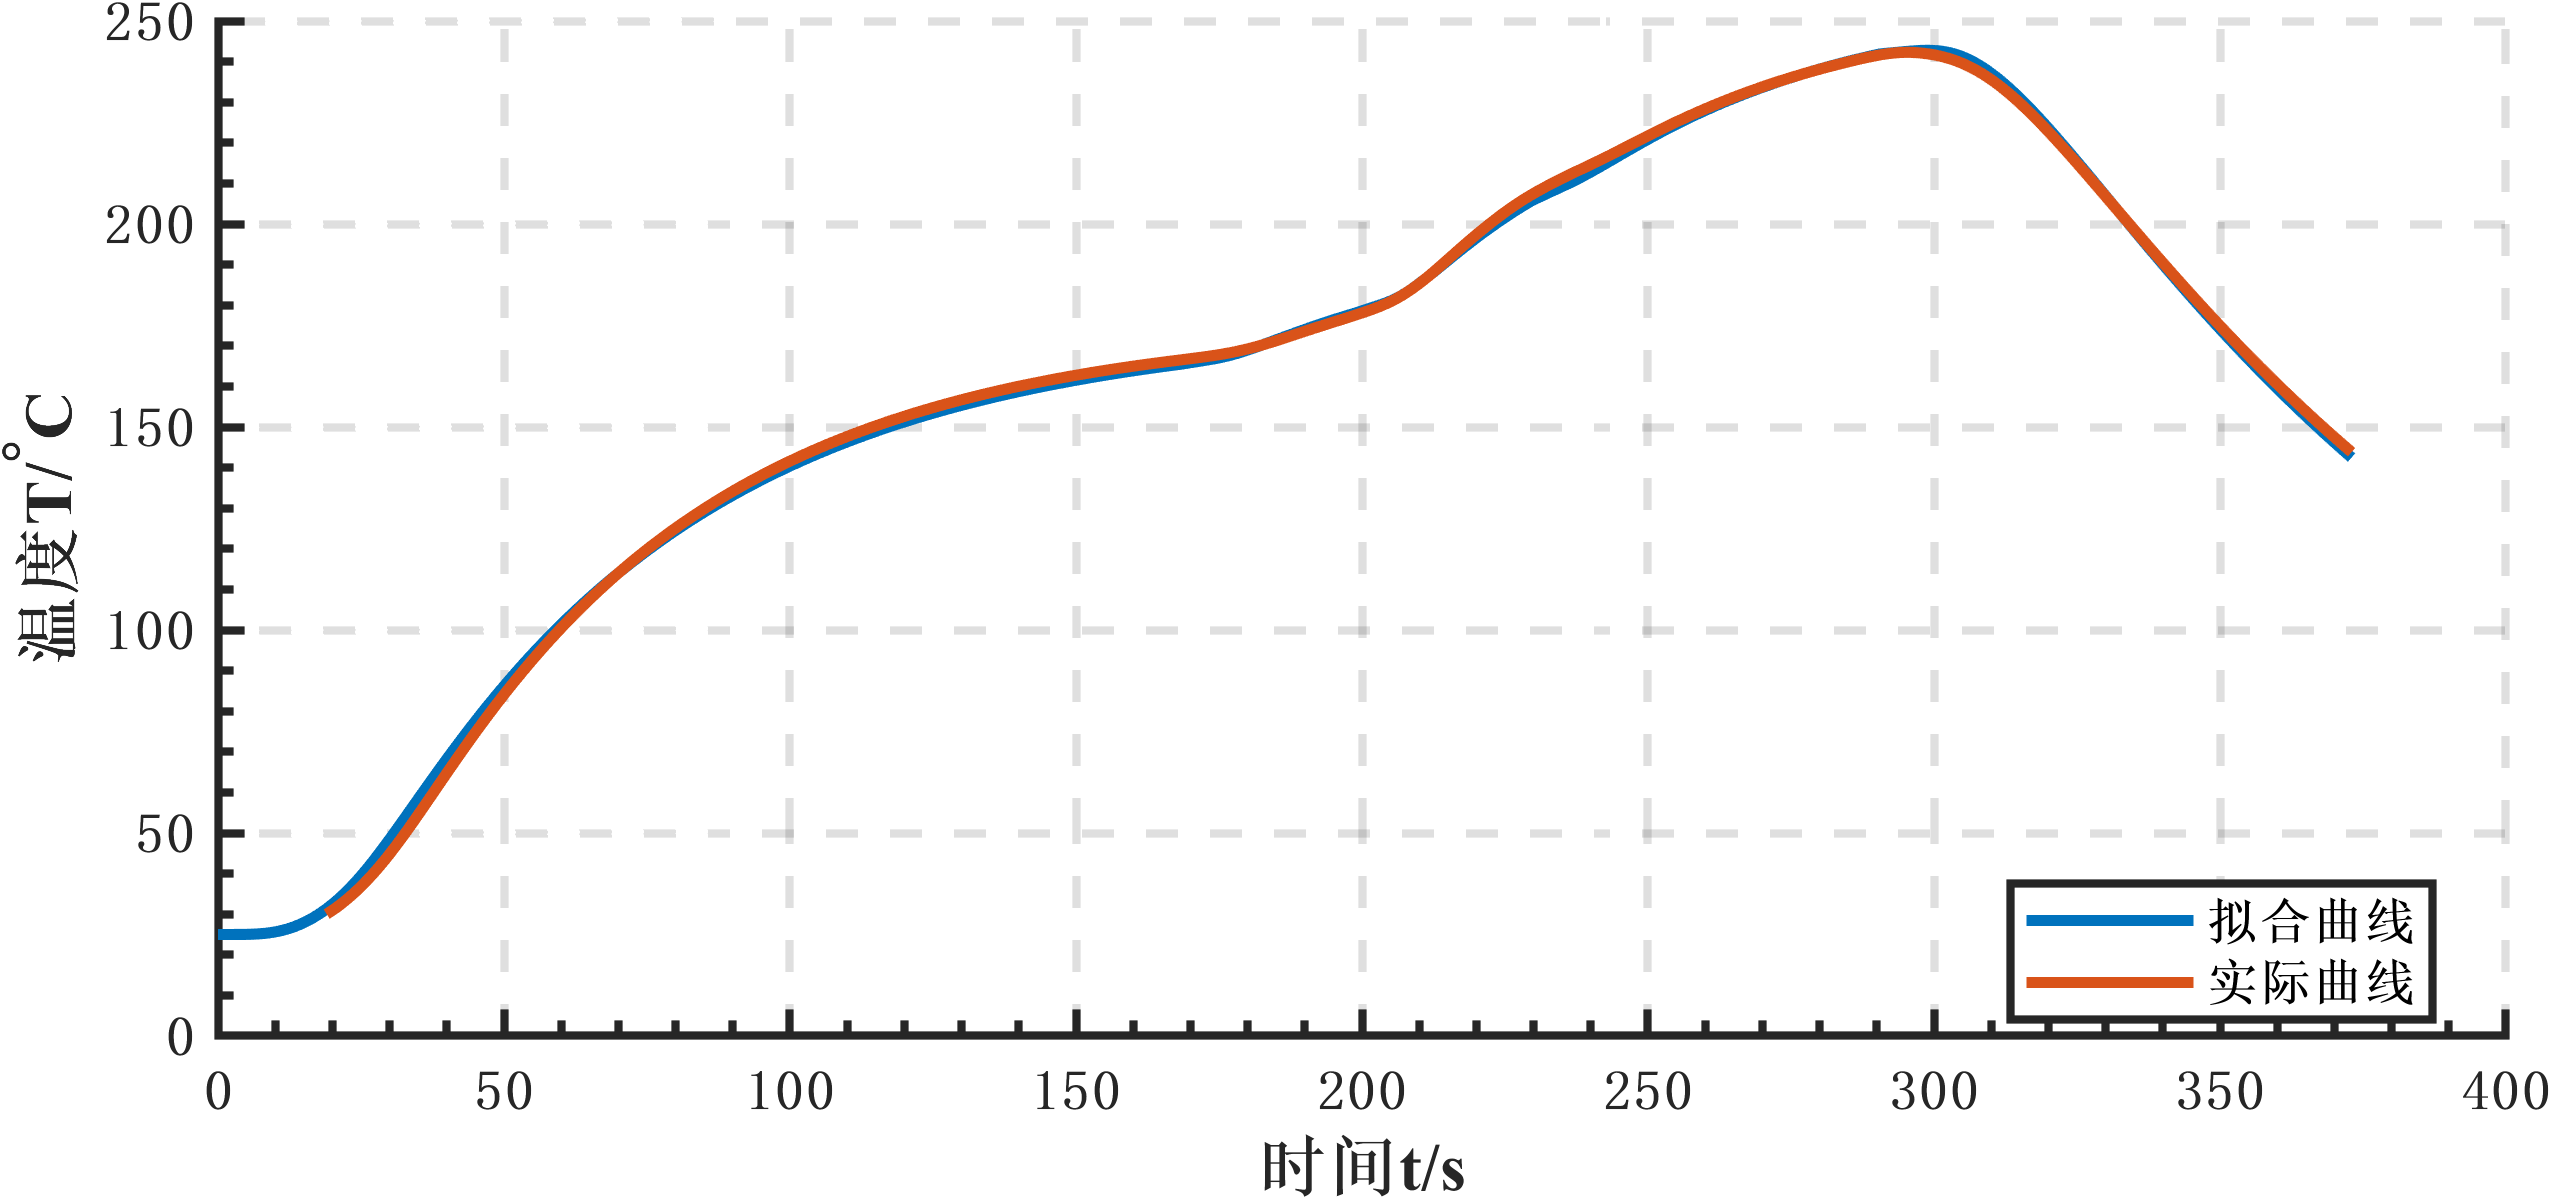
\includegraphics[width=0.75\textwidth]{拟合}
		\caption{拟合炉温曲线与实际炉温曲线}
		\label{拟合}
	\end{figure}
	\subsection{问题一的求解}
	传送带过炉速度为78cm/min,各温区的温度分别为173ºC(小温区1~5)、198ºC(小温区6)、230ºC(小温区7)和257ºC(小温区8~9),将上述参数和求得的$\alpha,\beta$参数代入模型求解,得到炉温曲线如图\ref{问题1炉温曲线}
	\begin{figure}[H]
		\centering
		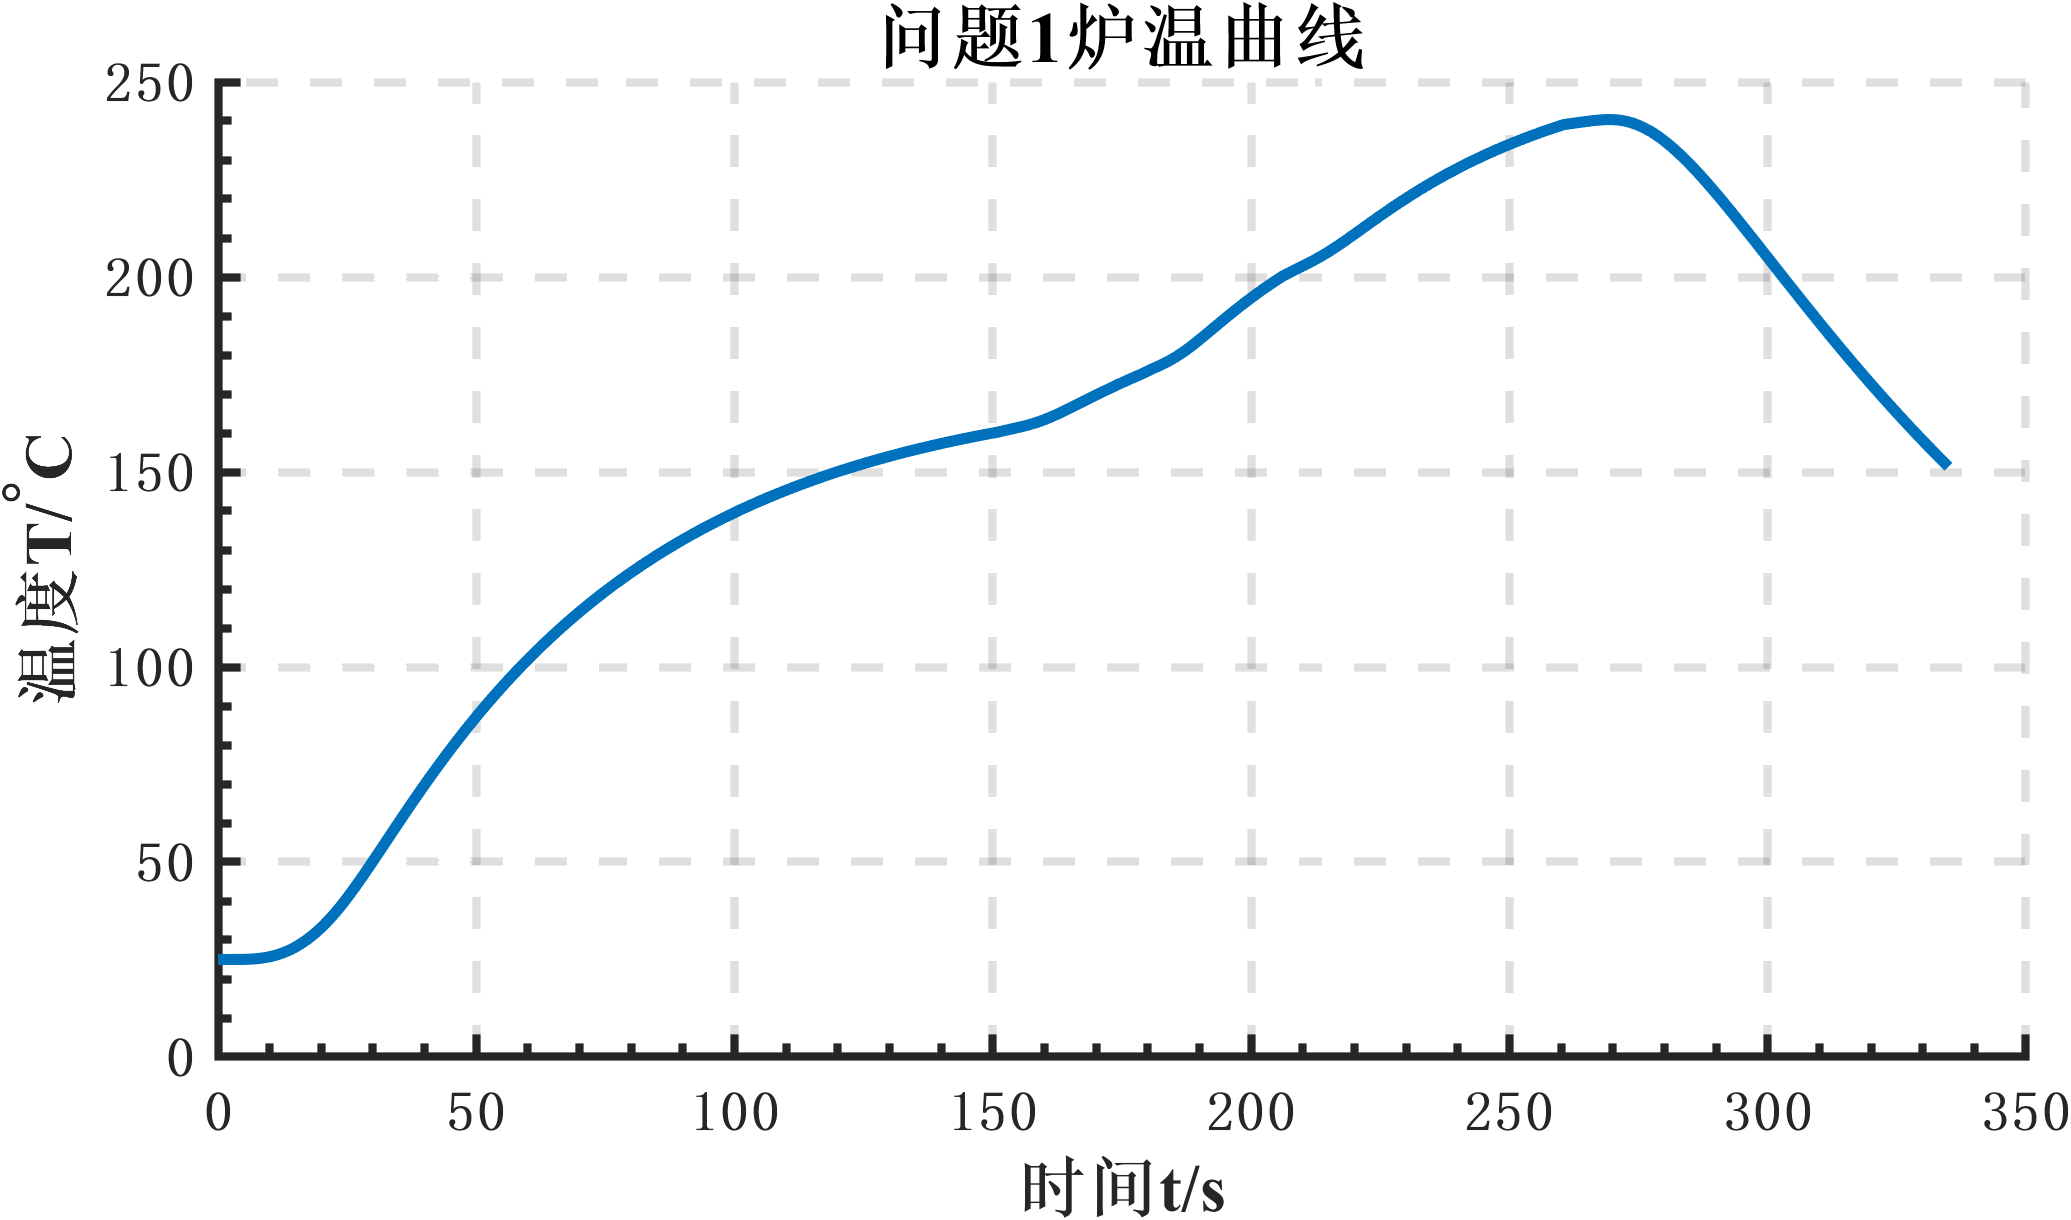
\includegraphics[width=0.75\textwidth]{问题1炉温曲线}
		\caption{问题1炉温曲线}
		\label{问题1炉温曲线}
	\end{figure}
	小温区3、6、7中点及小温区8结束处焊接区域中心的温度如表\ref{各点温度},每隔0.5 s焊接区域中心的温度已经存放在result.csv中。
	% Table generated by Excel2LaTeX from sheet '温区点温度'
	\begin{table}[htbp]
		\centering
		\caption{各点温度}
		\begin{tabularx}{\textwidth}{@{}c *3{>{\centering\arraybackslash}X}@{}}
			\toprule[1.5pt]
			 小温区3中点($^\circ C$)& 小温区6中点($^\circ C$) & 小温区7中点($^\circ C$)& 小温区8结束处($^\circ C$) \\
			 \midrule
			129.2787 & 168.2546 & 189.1527 & 231.5747 \\
			\bottomrule[1.5pt]
		\end{tabularx}%
		\label{各点温度}%
	\end{table}%
	\subsection{问题二模型的建立}
	问题二给出了各温区温度的设定值,其中小温区1~5为182ºC,小温区6为203ºC,小温区7为237ºC、小温区8-9为254ºC,需要求解在满足制程界限的前提下,允许的最大传送带过炉速度。以制程界限、热传导方程、空气温度随时间的变化函数、温区温度设定值为约束条件,以最大化传送带过炉速度为目标,建立单目标规划模型:

\begin{equation}\label{p2}
	\begin{gathered}
	\max\text{ }v
\\
\begin{cases}
\text{制程界限}\begin{cases}
\max \left( \left| \dot{u}\left( t \right) \right| \right) \leqslant 3\\
60\leqslant \left. t \right|\left( 150\leqslant u\left( t \right) \leqslant \text{190\&}\dot{u}\left( t \right) >0 \right) \leqslant 120\\
40\leqslant \left. t \right|\left( 217\leqslant u\left( t \right) \right) \leqslant 90\\
240\leqslant \max \left( u\left( t \right) \right) \leqslant 250\\
65<v<100\\
\end{cases}\\
\text{控制方程}\left\{ \begin{array}{l}
u(t)=u(\frac{d}{2},t)\\
\frac{\partial u\left( x,t \right)}{\partial t}=\alpha \frac{\partial ^2u\left( x,t \right)}{\partial x^2}\\
\left. \frac{\partial u}{\partial x} \right|_{x=d}=\beta \left( u_s\left( t \right) -u\left( d,t \right) \right)\\
-\left. \frac{\partial u}{\partial x} \right|_{x=0}=-\beta \left( u_s\left( t \right) -u\left( \text{0,}t \right) \right)\\
\end{array} \right.\\
\text{空气温度}u_s\left( t \right) =U_s=U_s\left( vt \right)\\
\text{温区温度}\begin{cases}
T_{15}=182\\
T_{06}=203\\
T_{07}=237\\
T_{89}=254\\
T_{1011}=25\\
\end{cases}\\
\end{cases}
	\end{gathered}
\end{equation}
\subsection{变范围搜索策略}
首先以$65cm/min$为初值,$1cm/min$为步长,$100cm/min$为终值,将各个参数代入模型求解炉温曲线,作出各制程的变化情况如图\ref{问题2各个指标随速度的变化}。
	\begin{figure}[H]
	\centering
	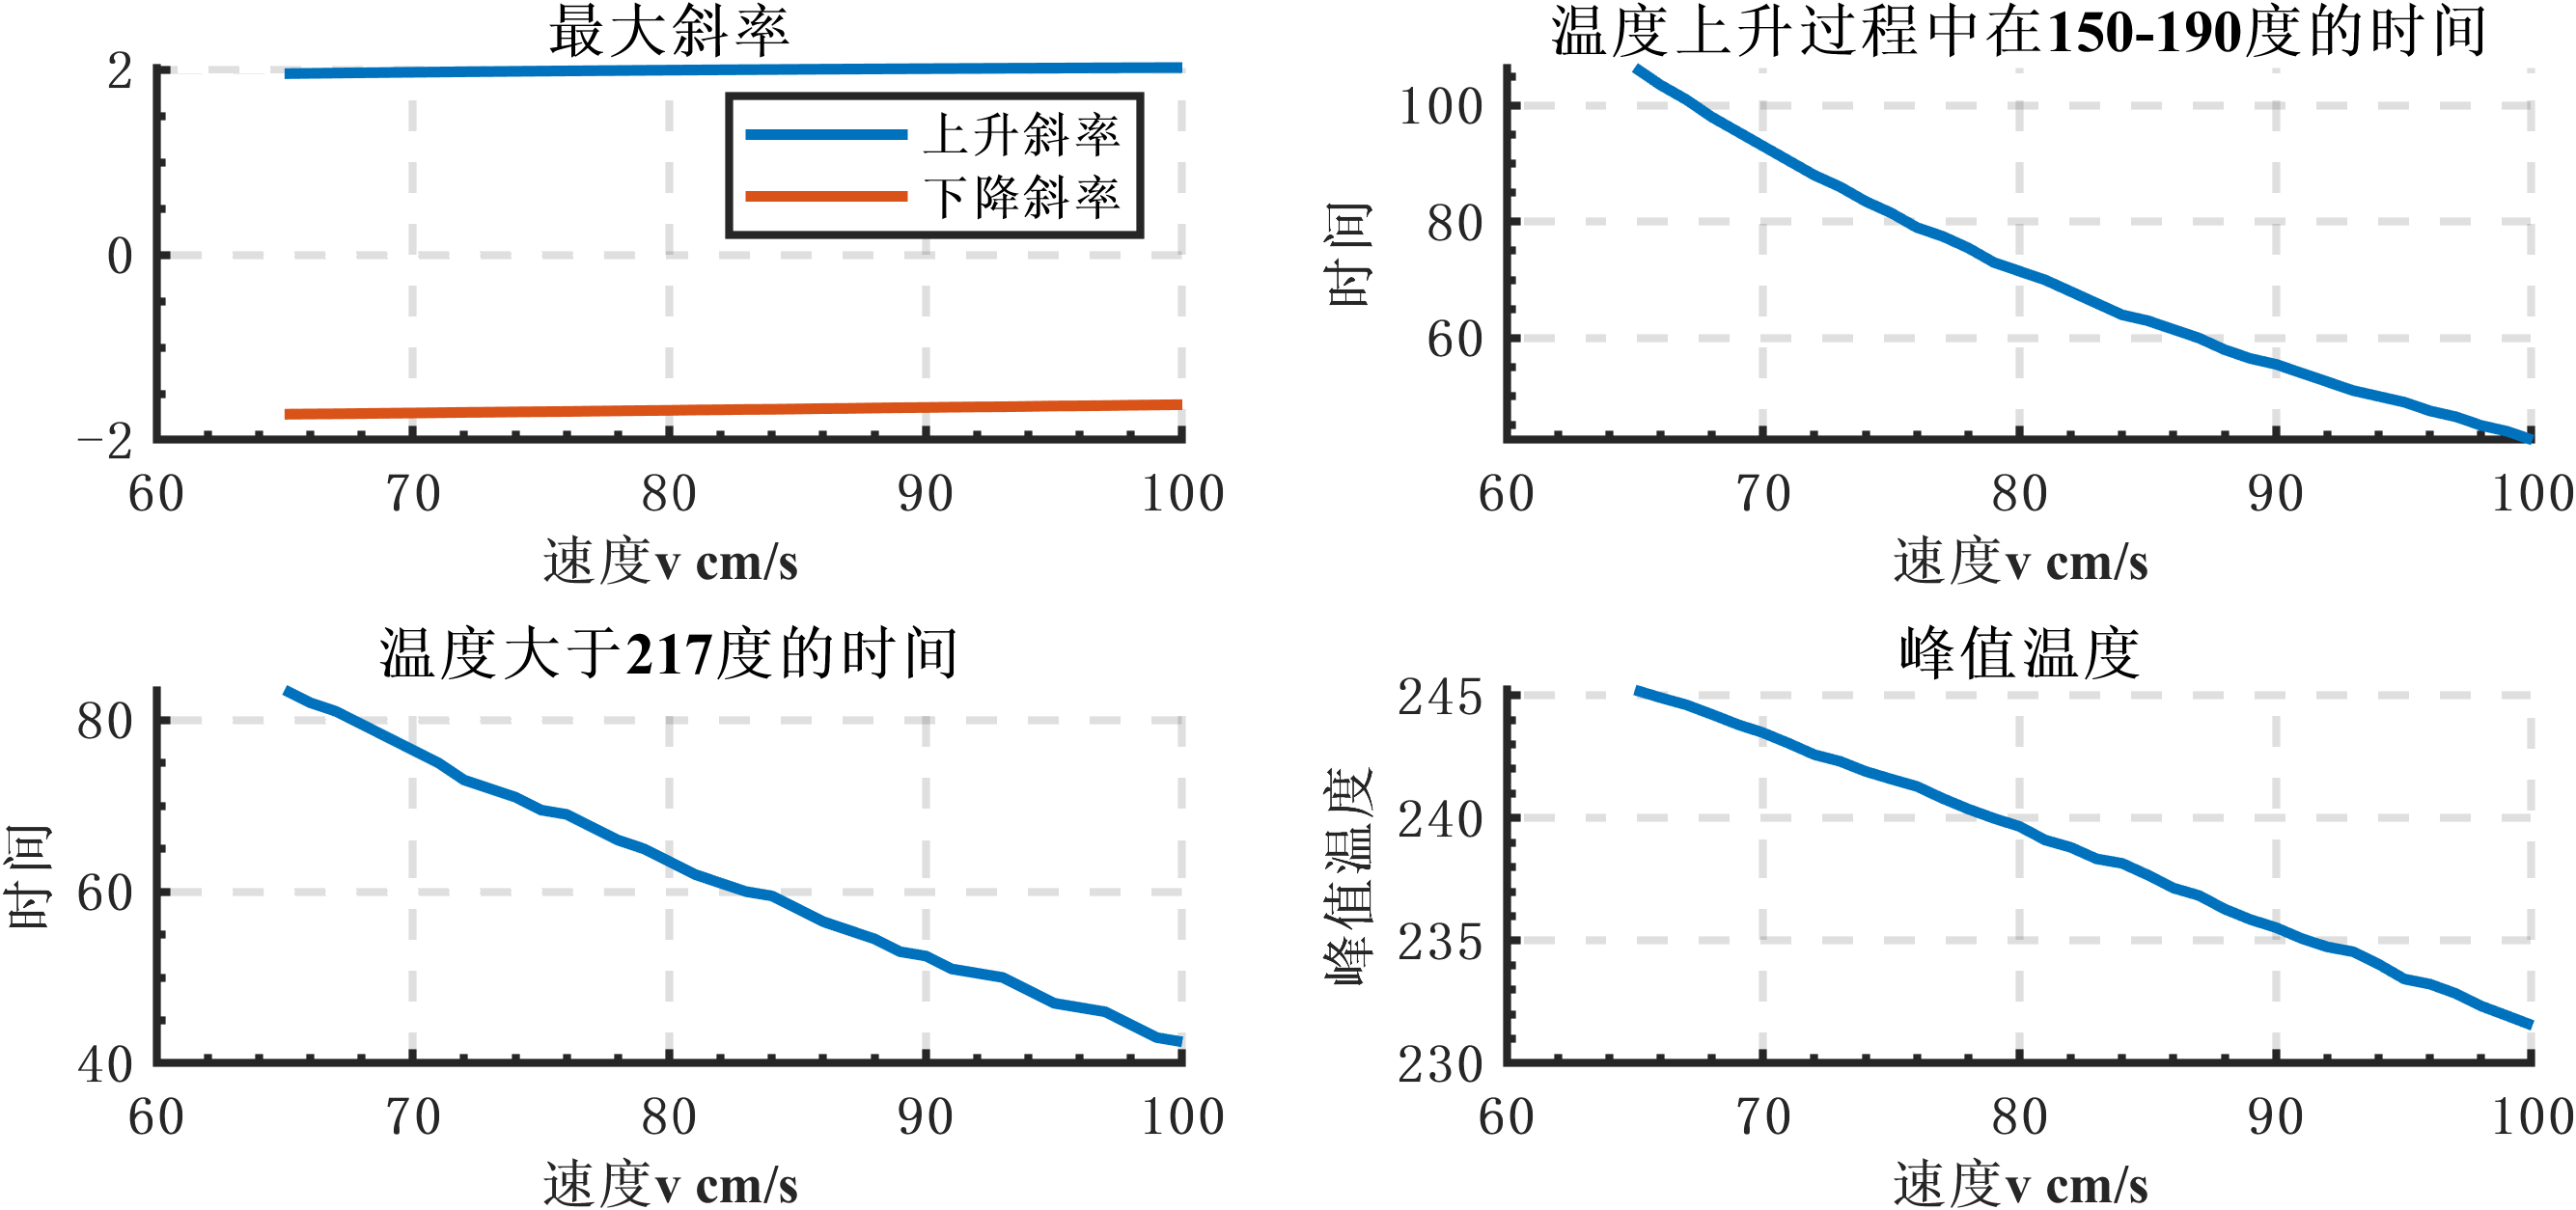
\includegraphics[width=0.75\textwidth]{问题2各个指标随速度的变化}
	\caption{问题2各个指标随速度的变化}
	\label{问题2各个指标随速度的变化}
\end{figure}
由图\ref{问题2各个指标随速度的变化}可以看出,速度在$65-100cm/min$时,斜率要求和温度大于217度的要求都满足,速度上升的过程中,温度上升过程中在150-190度的时间要求和峰值温度要求逐渐不满足,是速度的单调函数。由满足跳变到不满足时的速度为$78cm/min$,因此,缩小步长,以$0.01cm/min$的步长遍历$77-79cm/min$的速度,最终求得最大速度为$78.95cm/min$.
	
	\subsection{问题3模型的建立}
	问题3需要求解$[T_{15}, T_{06}, T_{0 7}, T_{89}, v]$,使得超过217ºC到峰值温度所覆盖的面积最小,并且满足制程及温度变化约束(上下波动10$^\circ C$)。面积可以通过积分求得,因此建立以面积最小化为目标的单目标规划模型:
\begin{equation}\label{p3}
\begin{gathered}
\left[\hat{T}_{15}, \hat{T}_{06}, \hat{T}_{07}, \hat{T}_{89}, \hat{v}\right]=\underset{T_{\mathrm{15}}, T_{06}, T_{0 7}, T_{89}, v} \arg \min S = \int_{t^{\prime}}^{t^{\prime \prime}}[u(t)-217] d t
\\
\begin{cases}
t^{\prime}=\min\text{\{}t\mid u\left( t \right) \ge \text{217\}}\\
t^{\prime \prime}=\underset{t}{arg}\,\,\max\text{ }u\left( t \right)\\
\text{制程界限}\begin{cases}
\max \left( \left| \dot{u}\left( t \right) \right| \right) \leqslant 3\\
60\leqslant \left. t \right|\left( 150\leqslant u\left( t \right) \leqslant \text{190\&}\dot{u}\left( t \right) >0 \right) \leqslant 120\\
40\leqslant \left. t \right|\left( 217\leqslant u\left( t \right) \right) \leqslant 90\\
240\leqslant \max \left( u\left( t \right) \right) \leqslant 250\\
65<v<100\\
\end{cases}\\
\text{控制方程}\left\{ \begin{array}{l}
u\left( t \right) =u\left( \frac{d}{2},t \right)\\
\frac{\partial u\left( x,t \right)}{\partial t}=\alpha \frac{\partial ^2u\left( x,t \right)}{\partial x^2}\\
\left. \frac{\partial u}{\partial x} \right|_{x=d}=\beta \left( u_s\left( t \right) -u\left( d,t \right) \right)\\
-\left. \frac{\partial u}{\partial x} \right|_{x=0}=-\beta \left( u_s\left( t \right) -u\left( \text{0,}t \right) \right)\\
\end{array} \right.\\
\text{空气温度:}u_s\left( t \right) =U_s=U_s\left( vt \right)\\
\text{速度界限:}65cm/\min \leqslant v\leqslant 100cm/\min\\
\text{温区温度界限}\begin{cases}
\left| T_{15}-175 \right|\leqslant 10\\
\left| T_{06}-195 \right|\leqslant 10\\
\left| T_{07}-235 \right|\leqslant 10\\
\left| T_{89}-255 \right|\leqslant 10\\
T_{1011}=25\\
\end{cases}\\
\end{cases}\\
\end{gathered}
\end{equation}
在求解面积$S$时,可以通过梯形法求解:
\begin{equation}
S=\sum_{i=i^{\prime}}^{i^{\prime \prime}-1} \frac{\Delta t}{2}\left[u((i-1) \Delta t)+u(i \Delta t)-2 u\left(i^{\prime}\right)\right]
\end{equation}
其中\begin{equation}
i^{\prime}=\left\lfloor\frac{t^{\prime}}{\Delta t}\right\rfloor+1, \quad i^{\prime \prime}=\left\lfloor\frac{t^{\prime \prime }}{\Delta t}\right\rfloor+1
\end{equation}
\subsection{遗传算法求解问题3单目标规划}
问题3是一个复杂的非线性规划问题,搜索变量有5个,分别是$[T_{15}, T_{06}, T_{0 7}, T_{89}, v]$,如果使用遍历的方法,花费的时间十分巨大。因此本文考虑使用遗传算法,以面积作为遗传算法的适应度函数,并使用罚函数法,将不满足温区温度界限的各温区温度、不满足速度界限的过炉速度、以及不满足制程界限的参数组合的适应度设置为一个很大的数(例如10000)。

为减少遗传算法的不确定性,增加说服力,多次使用遗传算法求解问题3,得到多组结果,如表\ref{问题3多组遗传算法求解结果}.其中某一次的算法收敛过程如图\ref{遗传算法过程图}.
% Table generated by Excel2LaTeX from sheet 'Sheet1'
\begin{table}[htbp]
	\centering
	\caption{问题3多组遗传算法求解结果}
	\begin{tabularx}{\textwidth}{@{}c *7{>{\centering\arraybackslash}X}@{}}
		\toprule[1.5pt]
		组别    & $T_{15} (^\circ C)$   & $T_{06} (^\circ C)$   & $T_{07}  (^\circ C)$  & $T_{89 }(^\circ C)$   & $v (cm/min)$     & 面积$S(^\circ C \cdot s)$   & 峰值温度$(^\circ C )$ \\
		\midrule
		1     & 184.1404 & 194.4357 & 240.5300 & 262.6221 & 94.1413 & 509.0461 & 240.0 \\
		2     & 182.1140 & 189.8592 & 230.2581 & 264.9846 & 91.5834 & 488.2102 & 240.0 \\
		3     & 177.9146 & 186.0785 & 230.9235 & 260.8567 & 84.2747 & 533.7085 & 240.0 \\
		4     & 183.1857 & 195.0097 & 233.7218 & 265.0000 & 94.7943 & 488.7792 & 240.0 \\
		5     & 179.8122 & 185.5750 & 239.1417 & 264.7966 & 94.0406 & 490.6426 & 240.0 \\
		6     & 174.3615 & 189.2047 & 236.8863 & 261.4947 & 87.7588 & 524.3180 & 240.0 \\
		7     & 170.3522 & 188.8334 & 226.1385 & 264.7179 & 86.5511 & 490.2605 & 240.0 \\
		8     & 173.7903 & 190.1923 & 229.6501 & 264.8884 & 89.3426 & 488.8328 & 240.0 \\
		9     & 181.8678 & 195.3838 & 231.2184 & 265.0000 & 92.8019 & 488.4086 & 240.0 \\
		10    & 174.0087 & 186.5502 & 232.0147 & 264.9075 & 89.8245 & 488.6447 & 240.0 \\
		\bottomrule[1.5pt]
	\end{tabularx}%
	\label{问题3多组遗传算法求解结果}%
\end{table}%
	\begin{figure}[H]
	\centering
	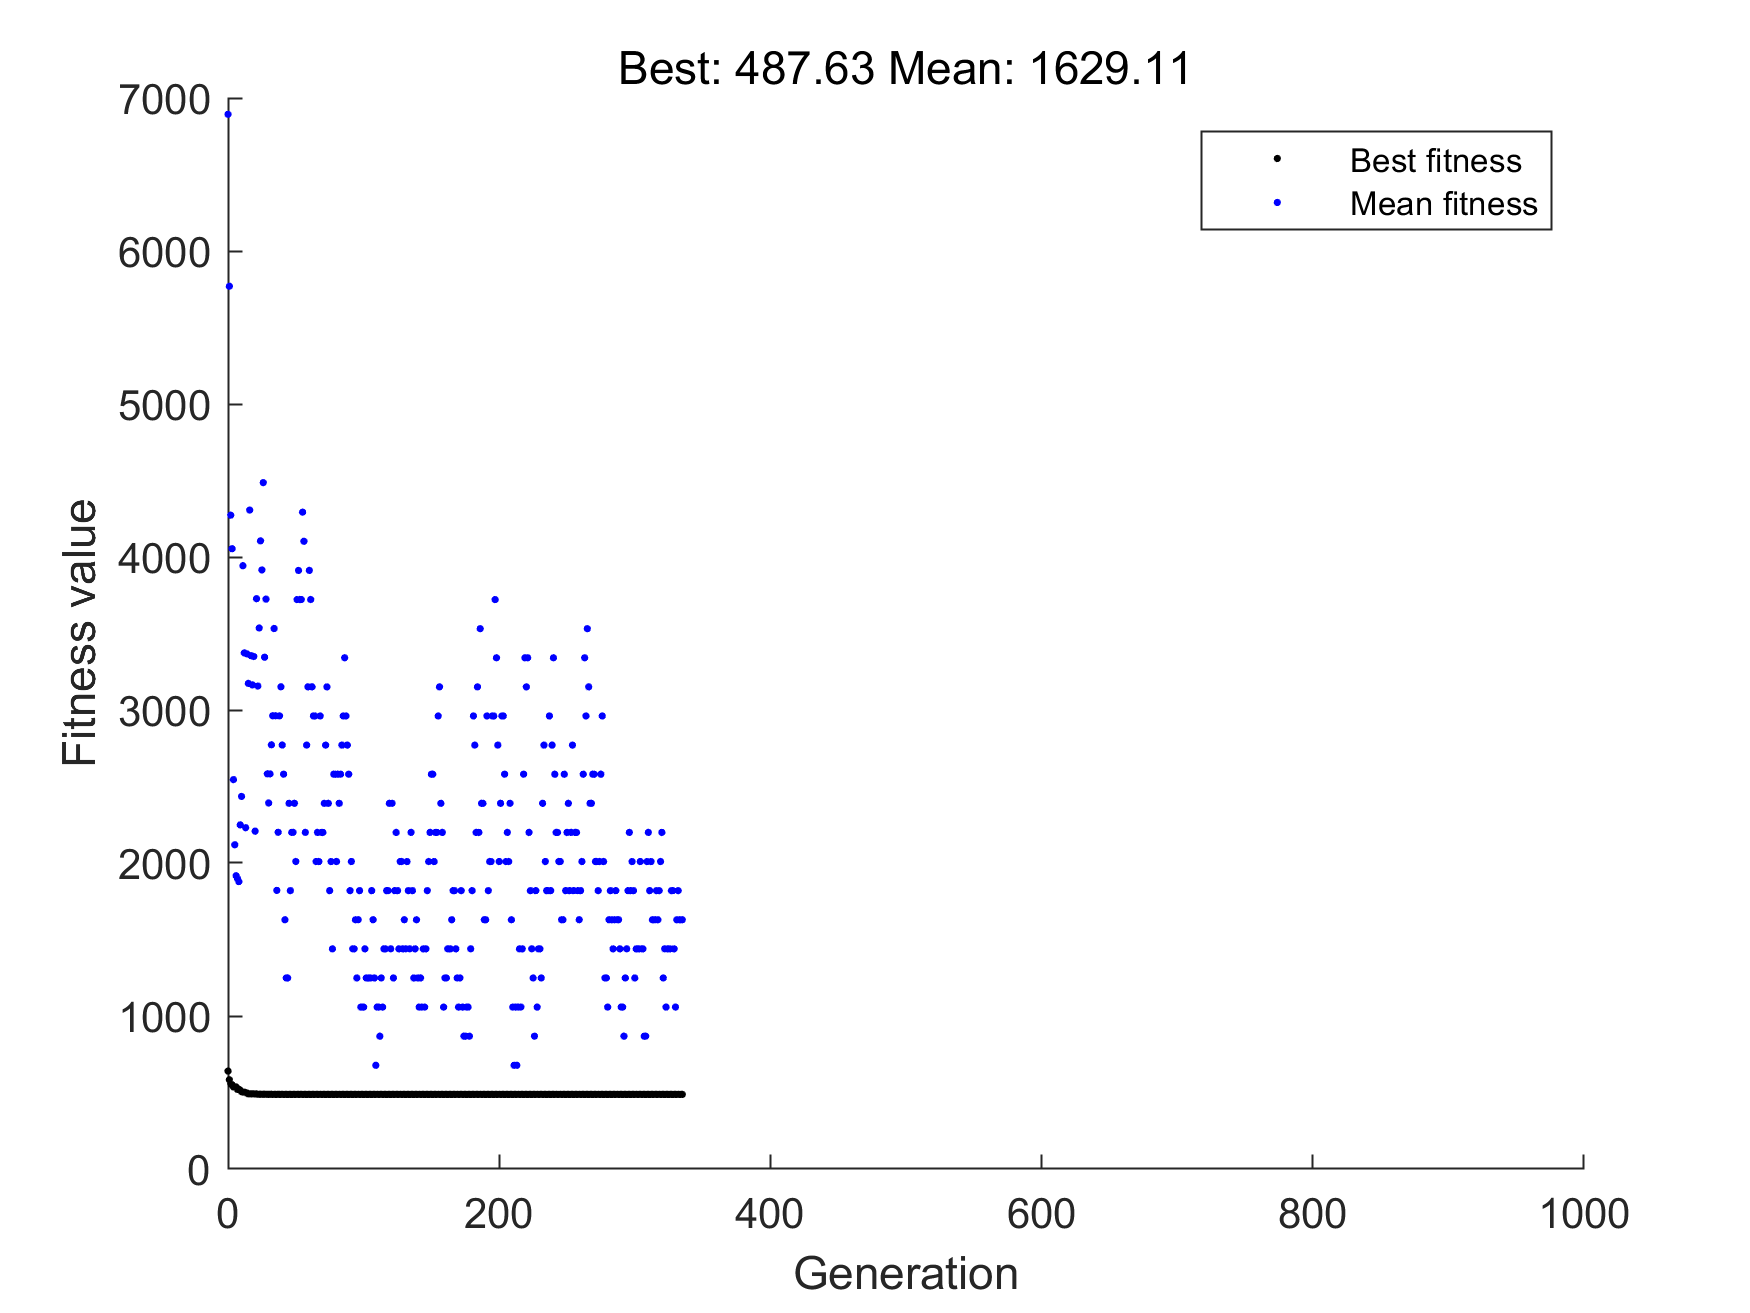
\includegraphics[width=0.65\textwidth]{遗传算法过程图}
	\caption{遗传算法过程图}
	\label{遗传算法过程图}
\end{figure}
可以看到,10次运行结果的峰值温度都是240$^\circ C$,即最小允许的峰值温度。因为峰值温度越大,面积相应地就会越大,为了得到最小的面积,因此需要峰值温度最小,模型的结果和我们的判断相符合。取面积最小的一次结果,即第2组的各个参数,作为问题3求解的最终参数,此时的面积指标为$488.2102(^\circ C \cdot s)$.

% Table generated by Excel2LaTeX from sheet 'Sheet1'
\begin{table}[htbp]
	\centering
	\caption{问题3最佳参数}
	\begin{tabularx}{\textwidth}{@{}c *4{>{\centering\arraybackslash}X}@{}}
		\toprule[1.5pt]
		$T_{15} (^\circ C)$   & $T_{06} (^\circ C)$   & $T_{07}  (^\circ C)$  & $T_{89 }(^\circ C)$   & $v (cm/min)$ \\
		\midrule
		182.1140 & 189.8592 & 230.2581 & 264.9846 & 91.5834 \\
		\bottomrule[1.5pt]
	\end{tabularx}%
	\label{tab:addlabel}%
\end{table}%
将最佳参数代入模型求解炉温曲线,如图\ref{问题3炉温曲线}.
	\begin{figure}[H]
	\centering
	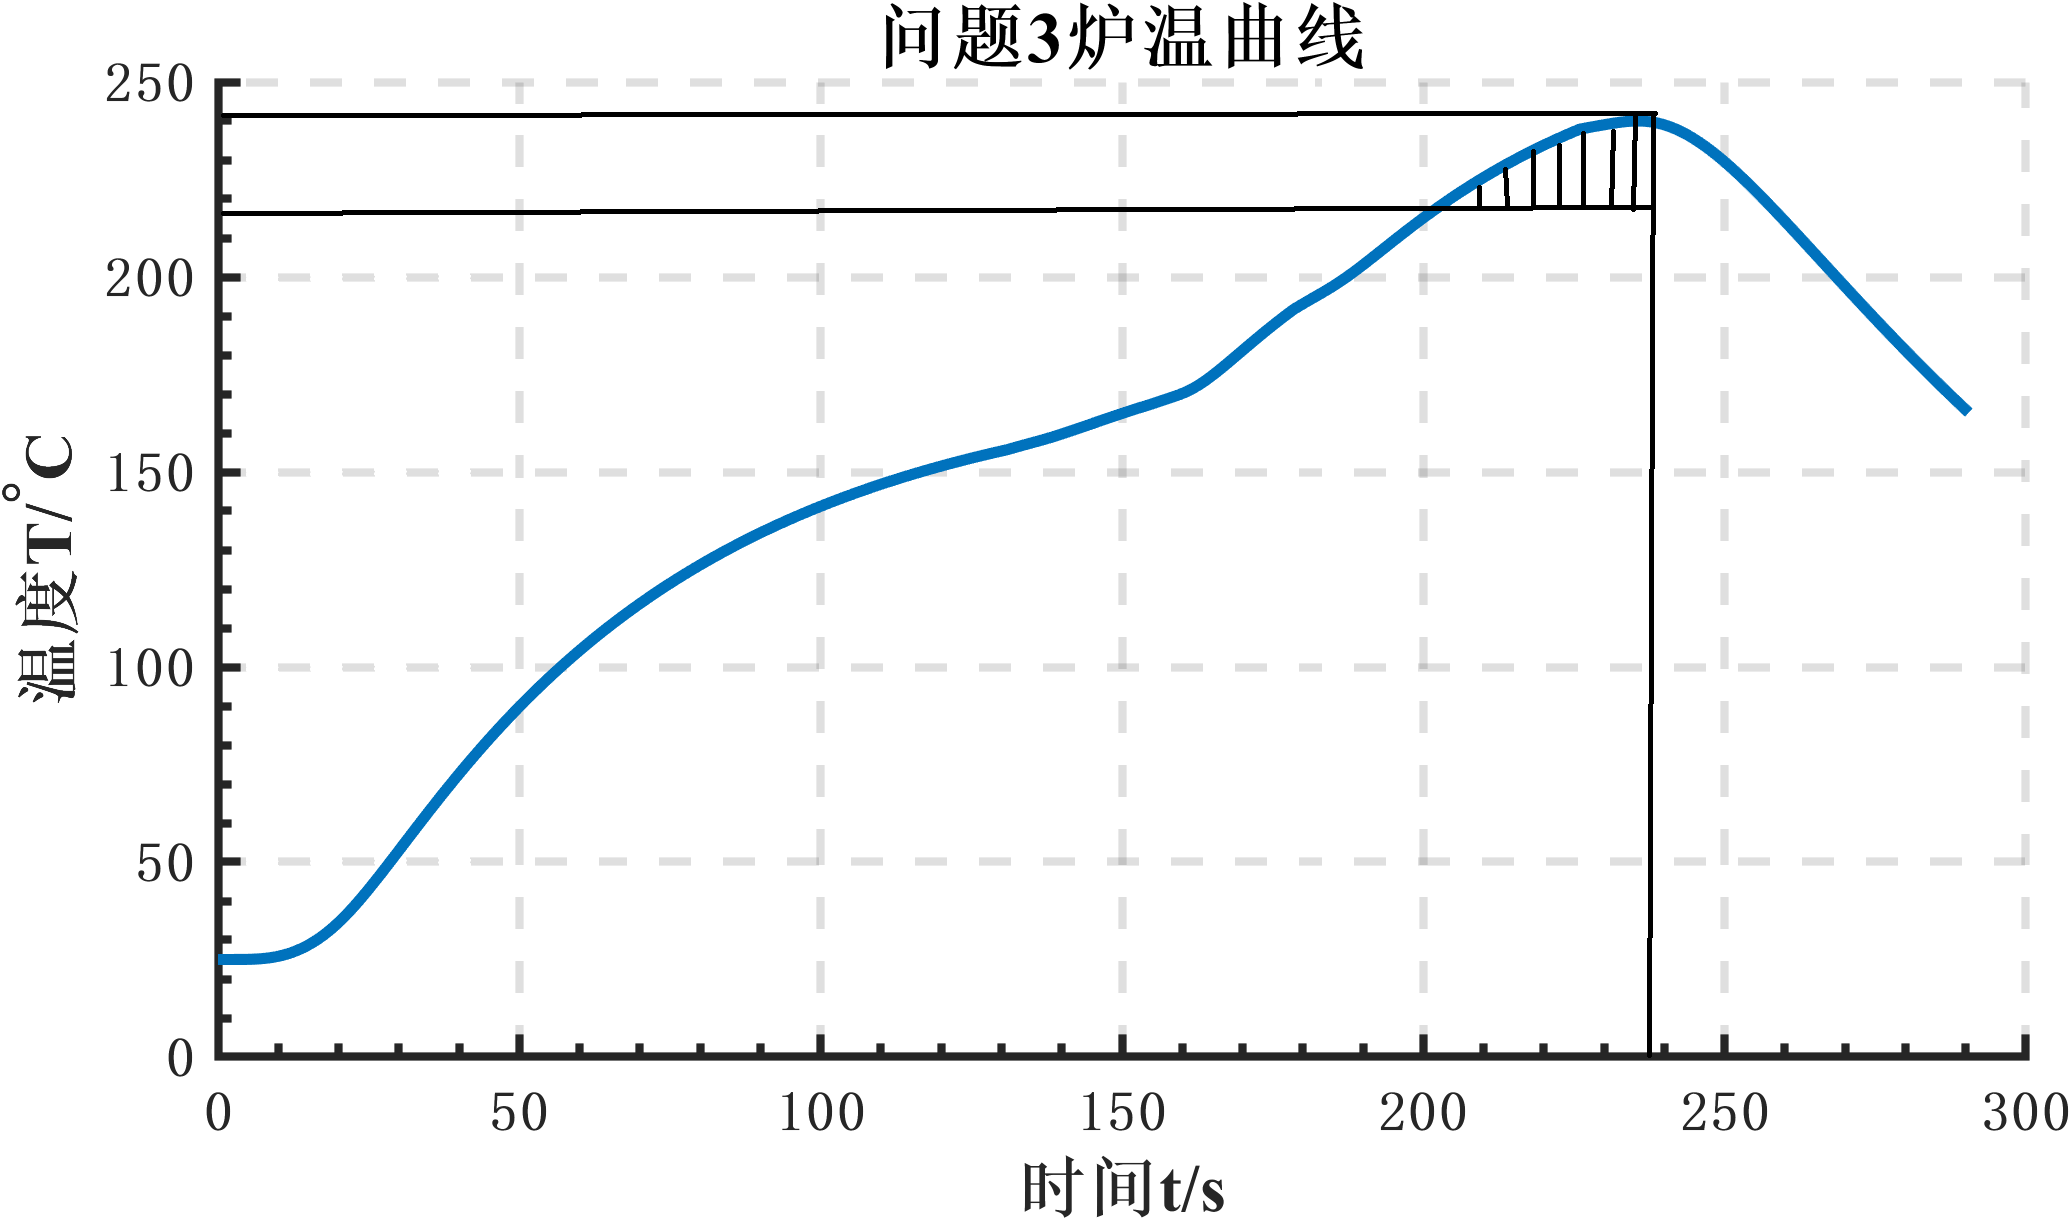
\includegraphics[width=0.70\textwidth]{问题3炉温曲线}
	\caption{问题3炉温曲线}
	\label{问题3炉温曲线}
\end{figure}

\subsection{问题4模型的建立}
$t^{\prime}=\min\text{\{}t\mid u\left( t \right) \ge \text{217\}}$为第一次到达217度的时刻,$t^{\prime \prime}=\underset{t}{arg}\max\text{ }u\left( t \right)$为峰值温度对应的时刻

定义$N=\frac{\lfloor t^{\prime \prime}-t^\prime \rfloor}{\Delta t}$为求和个数,对于大于$t^{\prime}$小于$t^{\prime \prime}$的时刻点$t^{\prime}+i\Delta t$,关于$t^{\prime \prime}$的对称点为$2 t^{\prime \prime}-i\Delta t$,两者作差并求和,得到关于对称性的指标$D$:
\begin{equation}\label{D}
D=\sqrt{\frac{1}{N}\sum_{i=0}^N{\left| u\left( 2t^{\prime\prime}-\left( t^\prime+i\Delta t \right) \right) -u\left( t^\prime+i\Delta t \right) \right|}^2}
\end{equation}
$D$越小,对称性越大。因此以面积$D$最小化和对称性指标$D$最小化为目标建立多目标规划模型:
\begin{equation}\label{p4}
\begin{gathered}
\left[ \hat{T}_{15},\hat{T}_{06},\hat{T}_{07},\hat{T}_{89},\hat{v} \right] =\underset{T_{15},T_{06},T_{07},T_{89},v}{arg}\min S= \int_{t^\prime}^{t^{\prime\prime}}{\left[ u\left( t \right) -217 \right]}dt
\\
\left[ \hat{T}_{15},\hat{T}_{06},\hat{T}_{07},\hat{T}_{89},\hat{v} \right] =\underset{T_{15},T_{06},T_{07},T_{89},v}{arg}\min D=\sqrt{\frac{1}{N}\sum_{i=0}^N{\left| u\left( 2t^{\prime\prime}-\left( t^\prime+i\Delta t \right) \right) -u\left( t^\prime+i\Delta t \right) \right|}^2}
\\
\begin{cases}
t^\prime=\min\text{\{}t\mid u\left( t \right) \ge \text{217\}}\\
t^{\prime\prime}=\underset{t}{arg}\,\,\max\text{ }u\left( t \right)\\
N=\frac{\lfloor t^{\prime\prime}-t^\prime \rfloor}{\Delta t}\\
\text{制程界限}\begin{cases}
\max \left( \left| \dot{u}\left( t \right) \right| \right) \leqslant 3\\
60\leqslant \left. t \right|\left( 150\leqslant Nu\left( t \right) \leqslant \text{190\&}\dot{u}\left( t \right) >0 \right) \leqslant 120\\
40\leqslant \left. t \right|\left( 217\leqslant u\left( t \right) \right) \leqslant 90\\
240\leqslant \max \left( u\left( t \right) \right) \leqslant \text{250,}65<v<100\\
\end{cases}\\
\text{控制方程}\left\{ \begin{array}{l}
u\left( t \right) =u\left( \frac{d}{2},t \right)\\
\frac{\partial u\left( x,t \right)}{\partial t}=\alpha \frac{\partial ^2u\left( x,t \right)}{\partial x^2}\\
\left. \frac{\partial u}{\partial x} \right|_{x=d}=\beta \left( u_s\left( t \right) -u\left( d,t \right) \right)\\
-\left. \frac{\partial u}{\partial x} \right|_{x=0}=-\beta \left( u_s\left( t \right) -u\left( \text{0,}t \right) \right)\\
\end{array} \right.\\
\text{空气温度:}u_s\left( t \right) =U_s=U_s\left( vt \right)\\
\text{速度界限:}65cm/\min \leqslant v\leqslant 100cm/\min\\
\text{温区温度界限}\begin{cases}
\left| T_{15}-175 \right|\leqslant \text{10,}\left| T_{06}-195 \right|\leqslant 10\\
\left| T_{07}-235 \right|\leqslant \text{10,}\left| T_{89}-255 \right|\leqslant 10\\
T_{1011}=25\\
\end{cases}\\
\end{cases}
\end{gathered}
\end{equation}
\subsection{分层序列法}
本文题中的模型有多个目标, 由于同时处理多个目标较为麻烦, 因此采用运筹学中的经典方法——分层序列法进行决策.

分层序列法的主体思想是根据各目标的重要程度依次排序, 分为最重要目标、次重要目标等, 对每个目标的最优解, 并以最优解的解集作为下一级目标的可行域, 再进行下一级目标的最优化, 直到所有目标优化完毕. 具体的算法过程如下:

设多个优化目标的优先级序列为:$f_{1}(x), f_{2}(x), \ldots, f_{m}(x)$ 首先对第一优先级目标$f_{1}(x)$求最优解, 并在该最优解集合$R_1$中求解第二优先级目标$f_{2}(x)$的最优解, 以此类方式逐个求解, 直至最后求$f_{m}(x)$最优解结束, 即为多目标问题的最优解集合$R_m$. 其有解的前提是$R_{0}, R_{1}, \ldots, R_{m-1}$非空, 且 $R_{0}, R_{1}, \ldots, R_{m-2}$至少有两个元素. 相对于常规的赋权优化方法,分层序列法性能优越, 且每步都有较为合适的现实含义与决策背景, 便于解决问题时与实际结合, 是一种有效的决策方法.

\subsection{使用结合分层序列法的遗传算法求解问题4}
对于问题4,可以使用结合分层序列法思想的遗传算法。步骤如下:

\textbf{Step1:}同问题3的求解过程,使用面积指标$S$作为遗传算法的适应度函数,对不满足条件的参数赋以较大的适应度,求解若干代后后保存最后的种群;

\textbf{Step2:}以步骤一中保存的种群为初始种群,使用对称性指标$D$作为遗传算法的适应度函数,使用罚函数法对不满足条件的参数赋以较大的适应度,同时求解面积指标$S$。在问题3中,求得的最小面积为$488.2102(^\circ C \cdot s)$,这里放宽限制,对$S>505^\circ C \cdot s$,本文认为其面积过大,同样使用罚函数法将这样的参数组合赋以较大的适应度,使其在进化的过程中被抛弃,对于面积$S<505^\circ C \cdot s$的参数组合,则留下参与进化。

\subsection{问题4求解结果}
同问题3,为减少遗传算法的不确定性,增加说服力,多次使用遗传算法求解问题,4,得到多组结果,如表\ref{q4b}.各组参数的两指标散点图如图\ref{问题4两指标散点图}.
	\begin{figure}[H]
	\centering
	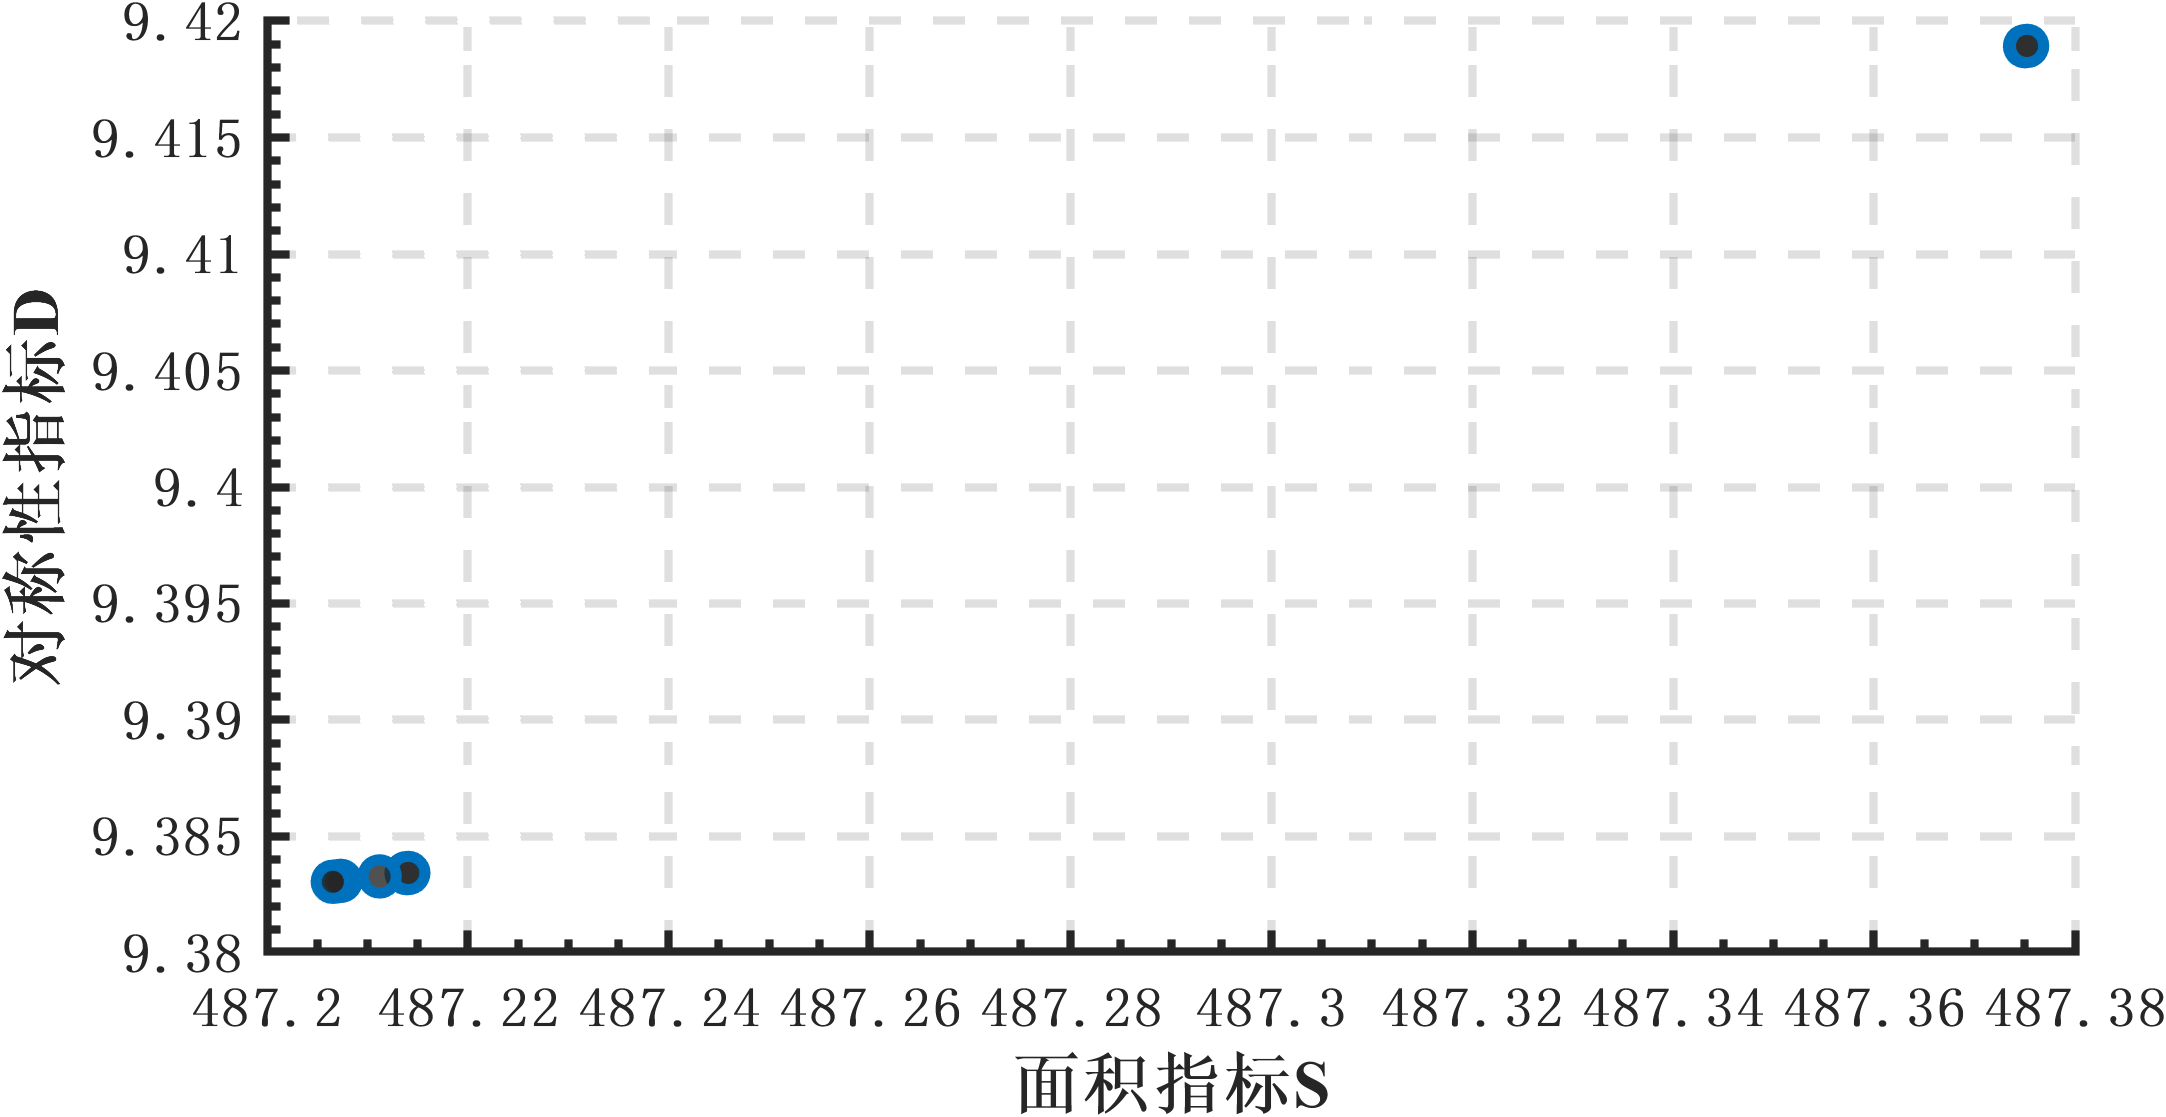
\includegraphics[width=0.70\textwidth]{问题4两指标散点图}
	\caption{问题4两指标散点图}
	\label{问题4两指标散点图}
\end{figure}
\begin{table}[htbp]
	\centering
	\caption{问题4遗传算法多次求解结果}
	\begin{tabularx}{\textwidth}{@{}c *7{>{\centering\arraybackslash}X}@{}}
		\toprule[1.5pt]
		组别    & $T_{15} (^\circ C)$   & $T_{06} (^\circ C)$   & $T_{07}  (^\circ C)$  & $T_{89 }(^\circ C)$   & $v (cm/min)$     & 面积指标$S(^\circ C \cdot s)$   & 对称性指标$(^\circ C )$ \\
		\midrule
		1     & 172.9719 & 185.2241 & 230.2076 & 265   & 88.7127 & 487.2139 & 9.3834 \\
		2     & 172.3227 & 185.1239 & 230.591 & 265   & 88.7126 & 487.2074 & 9.3831 \\
		3     & 172.3448 & 185.027 & 230.6251 & 265   & 88.7125 & 487.2068 & 9.3831 \\
		4     & 172.3717 & 185.0462 & 230.6021 & 265   & 88.7125 & 487.2072 & 9.3831 \\
		5     & 172.8574 & 185.0523 & 231.9734 & 265   & 88.9720 & 487.3750 & 9.4189 \\
		6     & 172.8416 & 185.0936 & 231.9621 & 265   & 88.9720 & 487.3752 & 9.4189 \\
		7     & 172.3051 & 185.0758 & 230.6227 & 265   & 88.7127 & 487.2068 & 9.3831 \\
		8     & 172.5251 & 185.748 & 230.1928 & 265   & 88.7125 & 487.2141 & 9.3834 \\
		9     & 172.5383 & 185.3709 & 230.3632 & 265   & 88.7125 & 487.2112 & 9.3833 \\
		10    & 172.3431 & 185.0034 & 230.637 & 265   & 88.7126 & 487.2066 & 9.3831 \\
		\bottomrule[1.5pt]
	\end{tabularx}%
	\label{q4b}%
\end{table}%
由于两个目标函数都是最小化目标函数,因此可以取散点图中最靠近原点的参数组合,即两个目标函数值都最小的参数组合,显然,第10组参数组合两目标函数都是最小,因此,取第10组参数作为最佳参数,代入模型求解炉温曲线,并与实验数据对比,如图\ref{问题4炉温曲线},显然,本文模型求解的炉温曲线与实验数据相比,具有很好的对称性。

综上,问题4最佳参数组合如下,其中面积为487.2066$S(^\circ C \cdot s)$,对称性指标为9.3831$(^\circ C )$。
\begin{table}[htbp]
	\centering
	\begin{tabularx}{\textwidth}{@{}c *4{>{\centering\arraybackslash}X}@{}}
		\toprule[1.5pt]
		$T_{15} (^\circ C)$   & $T_{06} (^\circ C)$   & $T_{07}  (^\circ C)$  & $T_{89 }(^\circ C)$   & $v (cm/min)$    \\
		\midrule
		172.3431 & 185.0034 & 230.637 & 265   & 88.7126 \\
		\bottomrule[1.5pt]
	\end{tabularx}%
	\label{tab:addlabel}%
\end{table}%

	\begin{figure}[H]
	\centering
	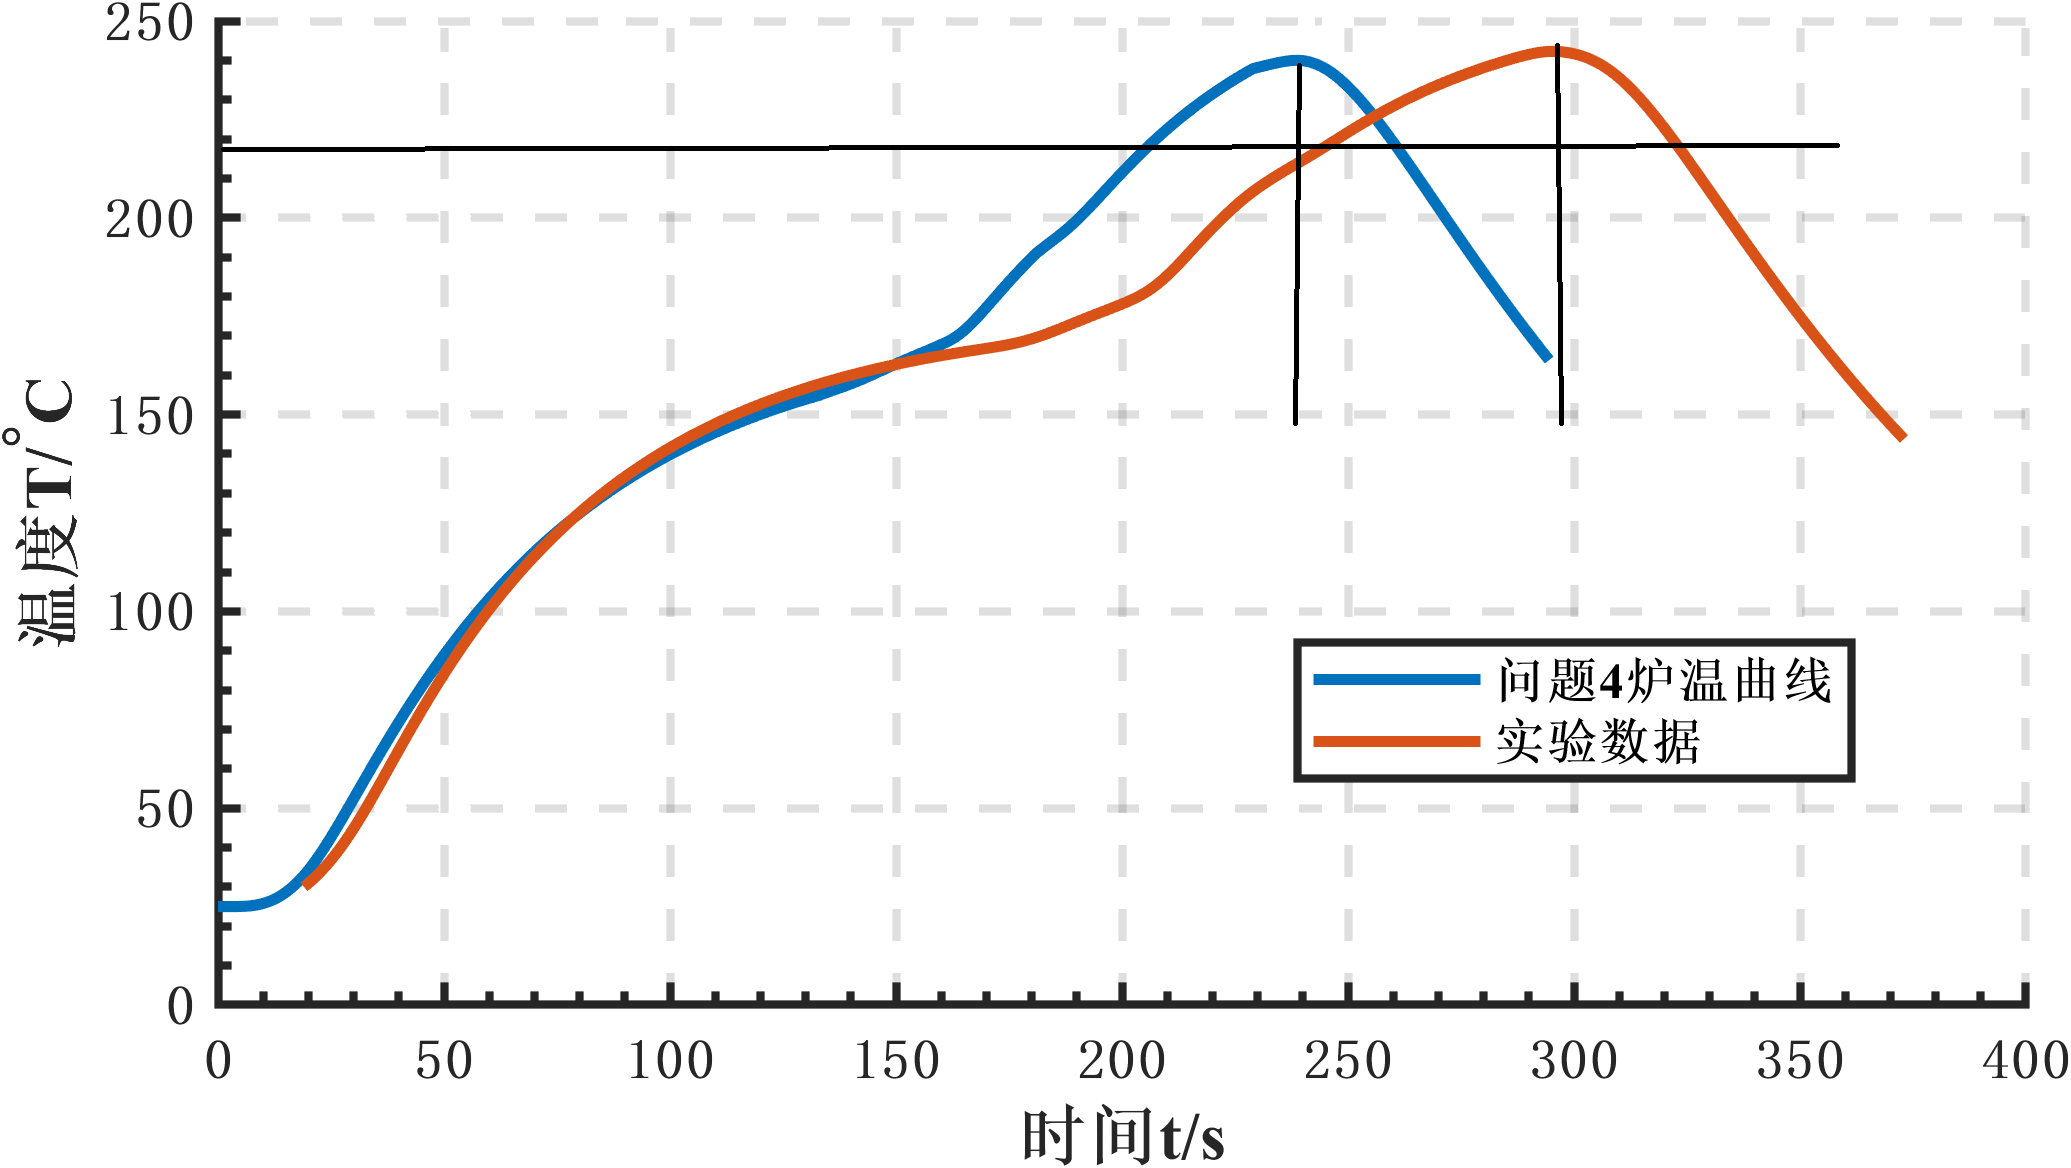
\includegraphics[width=0.70\textwidth]{问题4炉温曲线}
	\caption{问题4炉温曲线对称性与实验数据对比}
	\label{问题4炉温曲线}
\end{figure}

	\section{灵敏性分析}
	对于问题3,本文求得了最佳温区温度和最佳速度,考虑到实际需要控制的温度十分严格,精度需要达到0.1$^\circ C$,因此,对小温区1-5的温度$T_{15}$,小温区6的温度$T_{06}$,小温区7的温度$T_{07}$,小温区8、9的温度$T_{89}$在最佳温度附近施加以0.1$^\circ C$为步长的正负变化,并计算相应的面积$S$的改变量,如图\ref{灵敏度分析}
		\begin{figure}[H]
		\centering
		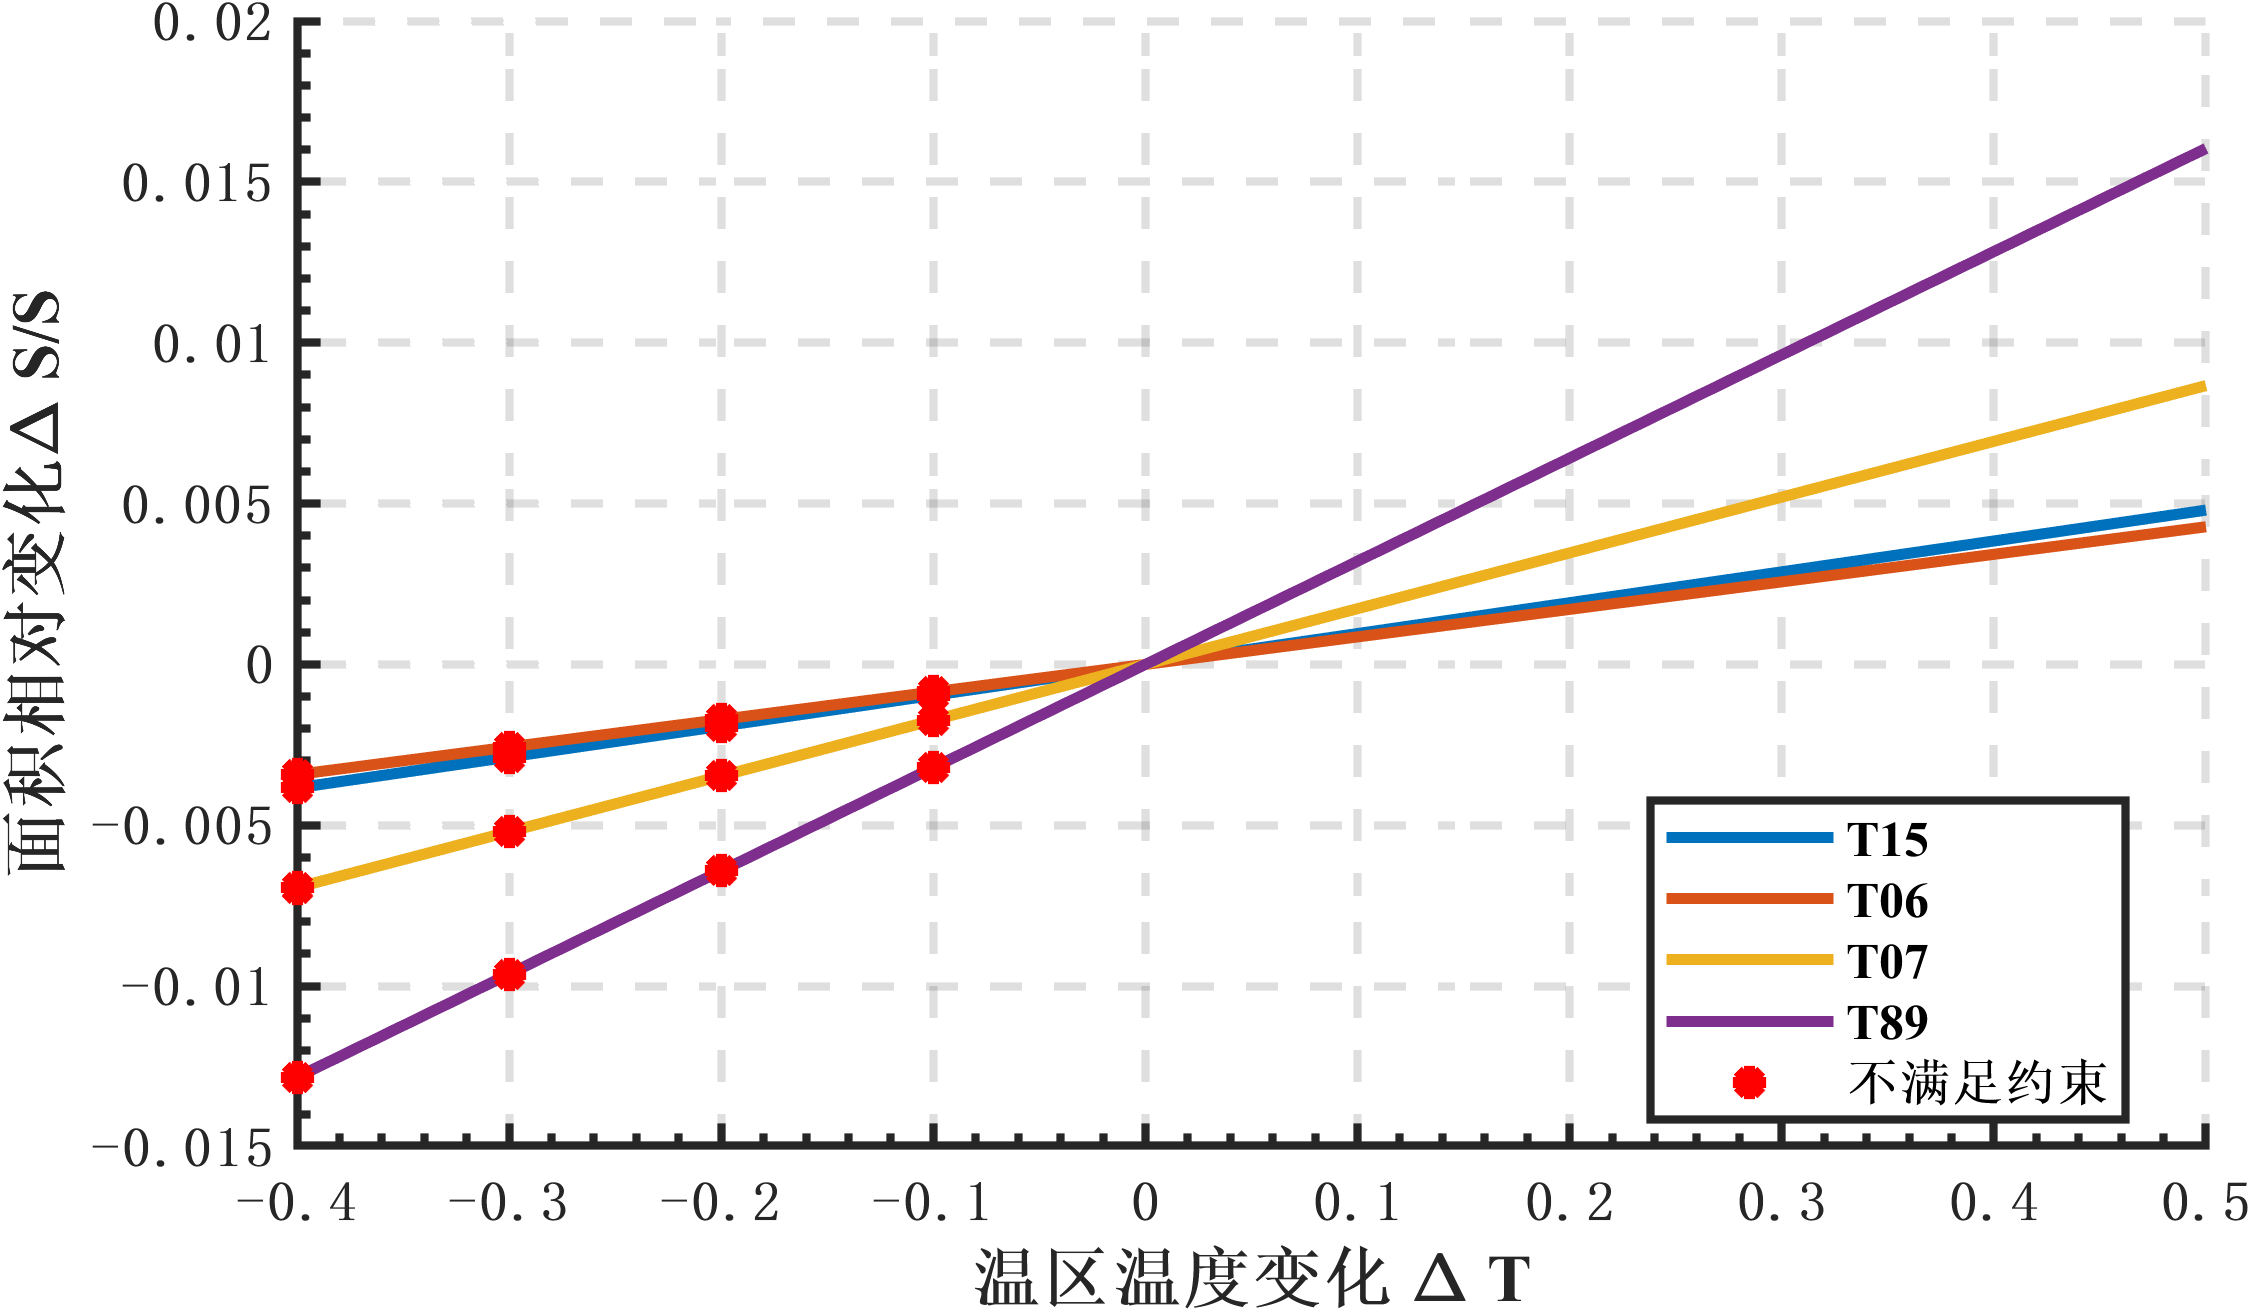
\includegraphics[width=0.70\textwidth]{灵敏度分析}
		\caption{灵敏度分析}
		\label{灵敏度分析}
	\end{figure}
	可以看到,改变各温区温度值,面积$S$的改变量在$-1.5\%-2\%$之间。当温度上升时,面积变大,当温度下降时,面积变小但是不满足制程约束。可见面积对各温区温度较敏感,敏感程度由大到小依次是$T_{89},T_{07},T_{15},T_{06}$.在实际生产过程中,应该严格控制温度。

	\section{模型的评价}
	\subsection{模型的优点}
	\begin{itemize}
		\item 对回焊炉的热参数$\alpha$分段讨论,能够较准确地拟合实验数据,对炉温曲线的预测也更加精准;
		\item 对模型热参数$\alpha$和$\beta$的确定以及问题2的求解过程中,使用了变范围搜索的方法,减少了计算量,更快速地得到结果;
		\item 对问题3、4使用遗传算法,并结合分层序列法的思想,避免陷入局部最优,较好地解决了问题。
	\end{itemize}
	\subsection{模型的缺点}
	\begin{itemize}
		\item 未考虑热回收等对炉温曲线的影响;
		\item 问题3、4的求解时间较长。
	\end{itemize}
	%\subsection{模型的推广}
	
	%参考文献
	%	\begin{thebibliography}{9}%宽度9
	%		\bibitem[1]{liuhaiyang2013latex}
	%		刘海洋.
	%		\newblock \LaTeX {}入门\allowbreak[J].
	%		\newblock 电子工业出版社, 北京, 2013.
	%		\bibitem[2]{mathematical-modeling}
	%		全国大学生数学建模竞赛论文格式规范 (2020 年 8 月 25 日修改).
	%		\bibitem{3} \url{https://www.latexstudio.net}
	%	\end{thebibliography}
	
	%\section{参考文献}
	\nocite{*}
	%\addcontentsline{toc}{section}{参考文献}
	%\bibliographystyle{bib/gbt7714-2005}
	\bibliographystyle{gbt7714-numerical}
	%\bibliographystyle{unsrt}
	%\bibliographystyle{IEEEtran}
	\bibliography{bib/ref.bib}
	
	\newpage
	%附录
	\begin{appendices}
		\section{代码文件列表}
		% Table generated by Excel2LaTeX from sheet 'Sheet1'
		\begin{table}[htbp]
			\centering
		\begin{tabularx}{\textwidth}{@{}l *1{>{\centering\arraybackslash}X}@{}}
				\toprule[1.5pt]
				文件名   & 功能描述 \\
				\midrule
				Data.mat & 附件数据 \\
				getTs.m & 获取空气温度分布向量 \\
				getTt.m & 获取炉温曲线向量 \\
				find\_alpha\_beta\_ga.m & 寻找最佳参数值 \\
				problem1.m & 问题1求解 \\
				problem2.m & 问题2求解 \\
				problem3.m & 问题3求解 \\
				problem4.m & 问题4求解 \\
				condition.m & 根据温度向量判断是否满足制程约束 \\
				evaluateS.m & 计算面积指标 \\
				evaluateD.m & 计算对称性指标 \\
				linminxin.m & 灵敏性分析 \\
				alpha\_beta1.mat & 最佳热传导模型参数 \\
				problem3\_Data.mat & 问题3求解结果 \\
				problem4\_Data.mat & 问题4求解结果 \\
				\bottomrule[1.5pt]
			\end{tabularx}%
			\label{tab:addlabel}%
		\end{table}%
		
		\section{代码}
		getTs.m
		\lstinputlisting[language=matlab]{code/getTs.m}
		getTt.m
		\lstinputlisting[language=matlab]{code/getTt.m}
		find\_alpha\_beta\_ga.m
		\lstinputlisting[language=matlab]{code/find_alpha_beta_ga.m}
		problem1.m
		\lstinputlisting[language=matlab]{code/problem1.m}
		problem2.m
		\lstinputlisting[language=matlab]{code/problem2.m}
		problem3.m
		\lstinputlisting[language=matlab]{code/problem3.m}
		problem4.m
		\lstinputlisting[language=matlab]{code/problem4.m}
		condition.m
		\lstinputlisting[language=matlab]{code/condition.m}
		evaluateS.m
		\lstinputlisting[language=matlab]{code/evaluateS.m}
		evaluateD.m
		\lstinputlisting[language=matlab]{code/evaluateD.m}
		linminxin.m
		\lstinputlisting[language=matlab]{code/linminxin.m}
	\end{appendices}
	
\end{document} 